\documentclass[11pt,a4paper]{article}

% ── Packages ──────────────────────────────────────────────────
\usepackage[utf8]{inputenc}
\usepackage[T1]{fontenc}
\usepackage{graphicx}
\usepackage{booktabs}
\usepackage{amsmath,amssymb}
\usepackage{hyperref}
\usepackage[margin=2.5cm]{geometry}
\usepackage{caption}
\usepackage{subcaption}
\usepackage{xcolor}
\usepackage{enumitem}
\usepackage{multirow}
\usepackage{float}
\usepackage{cite}

\hypersetup{
    colorlinks=true,
    linkcolor=blue,
    citecolor=blue,
    urlcolor=blue,
}

% ── Title ─────────────────────────────────────────────────────
\title{\textbf{When LLMs Meet Citizens: \\Simulating and Predicting French Policy Attitudes\\with Large Language Models}}

\author{
    \large Haoran Hu\quad Junhao He\quad Yan Qiu\quad Lanxin Wei\\
    \normalsize Nanjing University
}

\date{\today}

\begin{document}
\maketitle

% ── Abstract ──────────────────────────────────────────────────
\begin{abstract}
Can large language models (LLMs) serve as plausible proxies for human respondents in public opinion research? This paper presents a systematic empirical investigation of LLM behavioral patterns in policy attitude simulation, using French retirement reform as a test case. Through three rounds of prompt ablation experiments (30,000 total LLM calls) and a controlled comparison of two sampling strategies (similarity-based retrieval vs.\ random sampling), we document four key regularities: (1) \textbf{prompt wording exerts outsized influence on LLM outputs}---the proportion supporting ``return to 62'' swung from 89\% to 29\% across three prompt iterations, a 60-percentage-point span driven solely by prompt design changes; (2) \textbf{similarity-based retrieval yields aggregate distributions closer to real survey benchmarks than random sampling} (gap to IFOP: +11.8pp vs.\ $-$17.6pp), challenging the intuition that random sampling is inherently more representative; (3) \textbf{at the individual level, age is the only substantively predictive feature} ($|$SHAP$|$=0.307), with all other demographic variables and text embeddings providing negligible additional predictive power---all feature engineering strategies and models converge to the same R$^2 \approx 0.28$ ceiling and classification Macro F1 $\leq$ 0.51; (4) this ceiling is driven by irreducible LLM sampling noise ($T=0.7$), not by insufficient features or data. Our contribution is a systematic empirical record of LLM behavioral regularities in polling simulation, and the finding that prompt design, sampling strategy, and semantic relevance play decisive roles under the current LLM paradigm.
\end{abstract}

% ================================================================
\section{Introduction}
% ================================================================

Public opinion polling is fundamental to democratic governance, yet traditional survey methods face mounting challenges: declining response rates, rising costs, and social desirability bias~\cite{groves2009survey}. The emergence of large language models (LLMs) with strong role-playing capabilities opens a new frontier: \textit{computational persona simulation}, where AI agents embodying diverse demographic profiles are queried for their attitudes on policy issues.

Existing research has largely focused on the binary question of whether LLMs can match real survey data. We argue that before answering ``can they?,'' the field needs a clearer empirical picture of \textbf{how LLMs actually behave} when simulating survey respondents: How does prompt design affect output distributions? Do sampling strategies introduce systematic bias? Which features drive individual-level predictions? These behavioral regularities form the factual basis for evaluating and improving LLM-based survey methodology.

This paper uses one of France's most contentious policy issues---the 2023 pension reform that raised the legal retirement age from 62 to 64---as a test case. Based on 6 million synthetic French personas and the DeepSeek-V4-Flash model, we conduct systematic experiments to document LLM behavioral patterns. Compared to prior work, this paper differs in three respects: (1) we conduct \textbf{three-round systematic prompt ablation}, changing one variable at a time to precisely measure its effect on output distribution; (2) we introduce a \textbf{controlled comparison of two sampling strategies} (similarity-based retrieval vs.\ random sampling) to test the causal role of semantic filtering; (3) we build a \textbf{dual-layer evaluation framework} that simultaneously examines LLM simulation at the aggregate (distributional) and individual (predictive) levels.

% ================================================================
\section{Related Work}
% ================================================================

\subsection{LLMs as Simulated Survey Respondents}

Recent work has explored using LLMs to simulate human participants in social science research. Argyle et al.~\cite{argyle2023out} demonstrated that GPT-3 can produce response patterns that resemble human survey data when conditioned on demographic backstories. Santurkar et al.~\cite{santurkar2023whose} showed that LLM outputs reflect certain demographic opinion patterns but systematically deviate on others. Park et al.~\cite{park2023generative} demonstrated that LLM agents can produce believable individual behaviors but not necessarily representative aggregate statistics. Our work extends this line by providing systematic prompt ablation results and a dual evaluation framework.

\subsection{Computational Political Science}

Machine learning has been applied to predict political attitudes from digital traces and survey data. Prior work focused on social media text~\cite{barbera2015tweeting}, voter file data~\cite{hersh2015hacking}, and traditional survey responses~\cite{montgomery2018predicting}. Our setting is unique: we predict \textit{simulated} attitudes from \textit{synthetically generated} persona texts, creating a closed experimental loop where we control both the predictor and target variables.

\subsection{Sentence Embeddings for Social Science}

Transformer-based sentence embeddings such as Sentence-BERT~\cite{reimers2019sentence} have been widely adopted for semantic textual similarity tasks. However, their ability to capture fine-grained sociopolitical signals---such as the difference between a supporter and opponent of a specific policy---remains underexplored. Our tests of text embedding predictive power directly address this gap.

% ================================================================
\section{Method}
% ================================================================

\subsection{System Architecture}

Our pipeline consists of four stages (Figure~\ref{fig:architecture}):

\begin{enumerate}[leftmargin=*]
    \item \textbf{Persona Generation:} A corpus of 6 million French personas is pre-generated, each containing 10 structured text fields (persona traits, cultural background, professional persona, sports/arts/travel/culinary interests, hobbies, career goals, skills) and 8 demographic attributes (age, sex, marital status, household type, occupation, education level, department, commune).
    \item \textbf{LLM Simulation:} For each selected persona, we construct a prompt combining demographic and persona information, send it through the DeepSeek-V4-Flash API (via SiliconFlow), and parse the response to extract a support score (0--10) and stance label (support/neutral/oppose).
    \item \textbf{Macro-Fitting:} Aggregated LLM response distributions are compared against IFOP survey benchmarks along multiple demographic dimensions.
    \item \textbf{Micro-Modeling:} Individual responses serve as targets for supervised ML models. Features are constructed from demographic attributes and persona text.
\end{enumerate}

\begin{figure}[H]
    \centering
    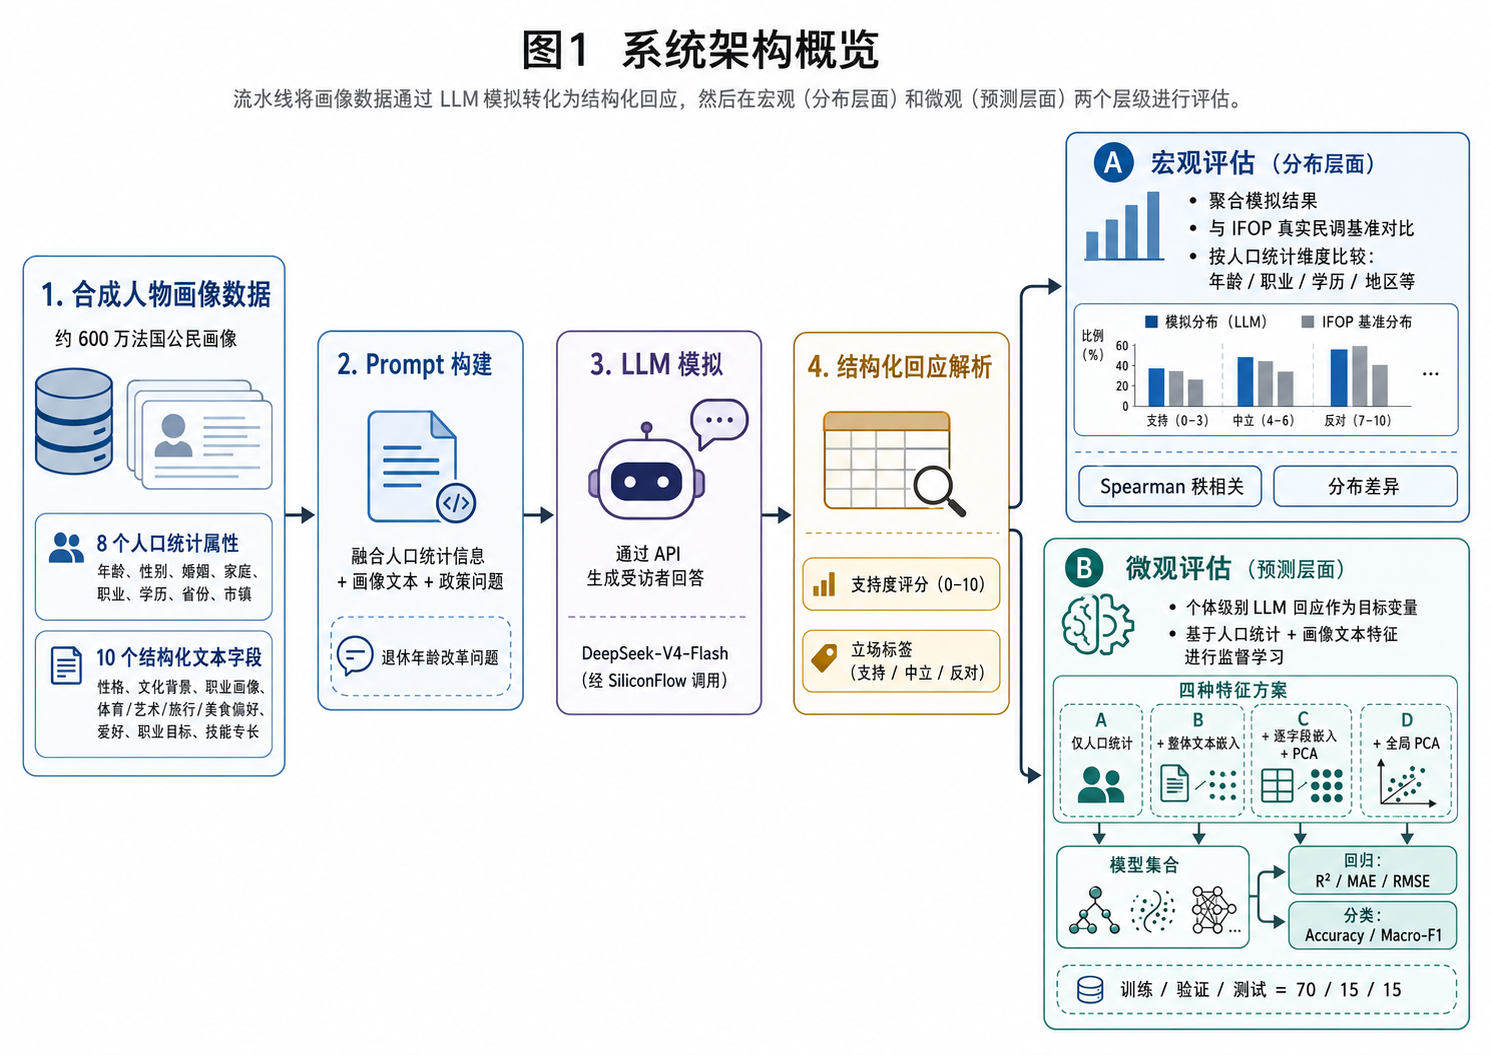
\includegraphics[width=0.85\textwidth]{figures/architecture.png}
    \caption{System architecture overview. The pipeline transforms persona data through LLM simulation into structured responses, then evaluates at both macro (distributional) and micro (predictive) levels.}
    \label{fig:architecture}
\end{figure}

\subsection{Persona Generation}

Each synthetic French citizen is described by 18 attributes across five categories: basic demographics (age, sex), socioeconomic status (occupation, education, marital status, household type), location (department, commune), personality profile (persona, cultural background, professional persona), and lifestyle (sports, arts, travel, culinary, hobbies, career goals, skills). The full dataset contains approximately 6 million unique personas stored in Parquet format (4.2 GB).

\subsection{Prompt Engineering: Three Iterations}

We conducted three systematic prompt iterations, each querying 10,000 personas with the same retirement reform question:

\begin{quote}
    \textit{关于法定退休年龄，您认为应该怎么做？回到62岁、维持在64岁，还是进一步提高？}
\end{quote}

Table~\ref{tab:prompt_iterations} summarizes the key differences across iterations and their results compared to the IFOP benchmark.

\begin{table}[H]
    \centering
    \caption{Prompt iteration comparison and alignment with IFOP benchmark}
    \label{tab:prompt_iterations}
    \begin{tabular}{@{}lcccc@{}}
        \toprule
        & \textbf{Run 1} & \textbf{Run 2} & \textbf{Run 3} & \textbf{IFOP} \\
        \midrule
        \textbf{Prompt design} & & & & \\
        \quad Persona guidance & Self-reference & +French context & Strictly persona & --- \\
        \quad Neutrality instruction & Avoid neutral & --- & --- & --- \\
        \quad Score mapping & No & No & Yes (0--10) & --- \\
        \quad Example provided & Yes & Yes & No & --- \\
        \midrule
        \textbf{Results (\%)} & & & & \\
        \quad Back to 62 & 89.0 & \textbf{72.8} & 28.9 & 61 \\
        \quad Maintain 64 & $\sim$10 & 17.9 & 70.9 & 34 \\
        \quad Further increase & $\sim$1 & 9.3 & 0.1 & 5 \\
        \midrule
        \quad Gap to IFOP & +28.0 pp & \textbf{+11.8 pp} & $-$32.1 pp & 0 \\
        \quad Mean score (0--10) & 6.87 & 6.29 & 5.78 & --- \\
        \bottomrule
    \end{tabular}
\end{table}

Run 2 achieved the closest alignment to real survey data. The key design elements were: (a) instructing the model to consider current French context while setting aside built-in values, (b) retaining a concrete example to anchor the response format, and (c) removing the explicit ``avoid neutrality'' instruction that pushed Run 1 toward extreme positions. Run 3 over-corrected by removing both the example and context instruction, causing responses to collapse into the neutral middle.

\subsection{LLM Simulation Setup}

All experiments use Run 2's prompt template as the baseline. The LLM API (DeepSeek-V4-Flash) was called through SiliconFlow with temperature = 0.7. Each response was parsed to extract a numerical support score (0--10, rescaled to 0--1 for regression) and a three-class stance label (support/neutral/oppose). The final dataset contains 8 demographic features, 10 text fields, and 2 target variables.

\subsection{Sampling Strategies: Similarity Retrieval vs.\ Random Sampling}

To test how sampling strategy affects LLM attitude simulation, we set up two controlled conditions:

\begin{enumerate}[leftmargin=*]
    \item \textbf{Similarity-based retrieval:} FAISS semantic search over SBERT embeddings of persona text, selecting the top-$K$ personas by cosine similarity to the retirement reform question embedding. This strategy filters for individuals whose persona descriptions contain retirement-, work-, or age-related semantic content, functionally analogous to a screening question in traditional surveys.
    \item \textbf{Random sampling:} Uniform random draw of $K$ personas from the full 6-million pool, with no topic-relevance constraints. This serves as the no-information-prior baseline.
\end{enumerate}

Both strategies use the identical question, prompt template (Run 2), and API parameters, with $K = 10{,}000$. The only difference is the sampling mechanism.

\subsection{ML Features and Models}

To examine the predictability of LLM attitude outputs at the individual level, we constructed four feature sets: \textbf{A} (8 demographic features, label-encoded); \textbf{B} (A + SBERT embedding of concatenated persona text, 8+384d); \textbf{C} (A + per-field PCA of 10 text fields, 16d each, concatenated, 8+160d); \textbf{D} (A + all 10 field embeddings concatenated to 3840d then globally PCA-reduced to 128d). All text embeddings use \texttt{all-MiniLM-L6-v2} (Sentence-BERT, 384-dimensional). Regression models include 11 variants (linear models, ensemble trees [Random Forest, XGBoost, LightGBM, CatBoost], SVR, MLP); classification covers 6 models (Logistic Regression, Gaussian Naive Bayes, Decision Tree, Random Forest, XGBoost, LightGBM), all with class weights to handle imbalance. Full configuration details are in the Appendix.

\subsection{Evaluation Protocol}

Data is split 70/15/15 (train/val/test) with stratification on stance labels. All four feature sets share identical split indices for fair comparison. We use 5-fold cross-validation on the training set and report final metrics on the held-out test set. Regression metrics: R$^2$, MAE, RMSE; classification metrics: Accuracy and Macro F1.

% ================================================================
\section{Results}
% ================================================================

\subsection{The Power of Prompts: From 89\% to 29\%}

The three-round prompt experiment (Table~\ref{tab:prompt_iterations}) reveals the extreme sensitivity of LLM attitude simulation to wording choices. Comparing Run 1 with Run 3, the proportion supporting ``return to 62'' dropped from 89\% to 29\%---a \textbf{60-percentage-point swing} driven solely by prompt design changes. For reference, real-world French opinion on retirement reform fluctuated by only 10--15 percentage points through months of national strikes, media debate, and political maneuvering. In other words, changing a prompt paragraph can produce a larger attitude distribution shift than a nationwide social movement.

Examining the marginal effect of each prompt element: Run 1 used an ``avoid neutrality'' instruction, which pushed 89\% of responses to the ``support'' extreme, nearly erasing neutral and oppose positions. Removing this instruction and adding ``consider the current French situation'' (Run 2) shifted the distribution meaningfully toward the center (support 72.8\%, neutral 17.9\%), reducing the IFOP gap from +28pp to +11.8pp. Further removing both the response example and contextual framing (Run 3) caused a wholesale collapse into neutrality (70.9\%), with support plunging to 29\%---despite the question itself being a clear value-laden choice. This collapse pattern suggests that, absent example anchoring and situational constraints, LLMs retreat to a ``safe'' neutral expression.

\subsection{Alignment and Misalignment with IFOP}

Run 2 achieved the closest aggregate alignment with IFOP (gap +11.8pp), but disaggregating by CSP occupational category reveals substantial heterogeneity (Table~\ref{tab:occupation_compare}).

\begin{table}[H]
    \centering
    \caption{Comparison of LLM simulation and IFOP survey by CSP occupational category (\% supporting ``Return to 62'')}
    \label{tab:occupation_compare}
    \begin{tabular}{@{}lccc@{}}
        \toprule
        \textbf{CSP Category} & \textbf{IFOP (\%)} & \textbf{LLM Run 2 (\%)} & \textbf{Gap (pp)} \\
        \midrule
        Ouvriers (Workers) & 73 & 61.4 & $-$11.6 \\
        Employ\'es (Employees) & 77 & 49.8 & $-$27.2 \\
        Professions interm\'ediaires (Intermediate) & 65 & 37.5 & $-$27.5 \\
        Cadres et prof. int. sup. (Executives) & 54 & 31.9 & $-$22.1 \\
        \bottomrule
    \end{tabular}
\end{table}

Two dimensions of deviation are notable. First, there is a \textit{ranking reversal}: in IFOP data, Employees (77\%) rank highest in support, followed by Workers (73\%), whereas the LLM places Workers (61.4\%) above Employees (49.8\%), suggesting the LLM may internalize a ``workers = most pro-reform'' stereotype while underestimating the depth of employee discontent. Second, the \textit{LLM systematically underestimates} support across all four CSP categories, with gaps ranging from $-$12 to $-$28pp. A structural contributor is sample composition bias: 56.6\% of LLM similarity-retrieved individuals fall into the CSP category ``Other without professional activity'' (Autres sans activit\'e professionnelle), which has no direct counterpart in the IFOP cross-tabulation and exhibits an extreme support rate of 95.6\% in the LLM simulation.

It bears noting that the ``benchmark'' itself is not bias-free. The IFOP survey (n=2,023) uses online self-administered questionnaires; its CSP classification is a statistical construct, and sampling quotas, non-response bias, and social desirability bias may all affect occupation-grouped accuracy. The LLM--IFOP gap should therefore not be simplistically equated with ``LLM error''---real survey data carries its own measurement uncertainty.

\subsection{Who Answers Matters: Similarity vs.\ Random}

As a methodological control, we tested random sampling without semantic filtering (Table~\ref{tab:sampling_comparison}).

\begin{table}[H]
    \centering
    \caption{Distribution comparison: similarity-based vs.\ random sampling}
    \label{tab:sampling_comparison}
    \begin{tabular}{@{}lccc@{}}
        \toprule
        & \textbf{IFOP} & \textbf{Similarity} & \textbf{Random} \\
        \midrule
        Support (back to 62) & 61\% & 72.8\% & 43.4\% \\
        Neutral (maintain 64) & 34\% & 17.9\% & 37.2\% \\
        Oppose (further increase) & 5\% & 9.3\% & 19.5\% \\
        \midrule
        Gap to IFOP (support) & --- & +11.8 pp & $-$17.6 pp \\
        \bottomrule
    \end{tabular}
\end{table}

The result is counterintuitive: random sampling, which intuition suggests should approximate an ``unbiased'' population distribution, in fact deviates \textit{more} from IFOP ($-$17.6pp) than similarity-based retrieval does ($+$11.8pp). A more balanced distribution (support/neutral/oppose = 43\%/37\%/20\%) did not translate into better benchmark alignment.

The mechanism behind this pattern: retirement reform is an issue with clearly defined stakeholder groups. Random sampling draws many individuals with no semantic connection to retirement (e.g., 20-year-old students, full-time parents). The LLM, lacking a semantic anchor for role-playing such personas, produces responses closer to ``guessing'' than ``reasoning,'' causing the distribution to drift away from real stakeholder attitudes. Similarity-based retrieval, while admittedly introducing selection bias toward issue-relevant individuals, performs a function analogous to a screening question in traditional surveys---identifying the relevant subpopulation before measuring attitudes. This suggests that \textbf{the notion of ``representativeness'' in LLM polling may need to shift from demographic balance toward semantic relevance}.

\subsection{Age Dominates Everything: SHAP Analysis}

To understand which features drive LLM attitude outputs at the individual level, we applied SHAP analysis to the XGBoost regression model under Approach C (demographics + per-field PCA), chosen because its field-name prefixes (e.g., persona\_pc*) make each PCA component traceable to its source text field (Figure~\ref{fig:feature_importance}).

\begin{figure}[H]
    \centering
    \begin{subfigure}{0.48\textwidth}
        \centering
        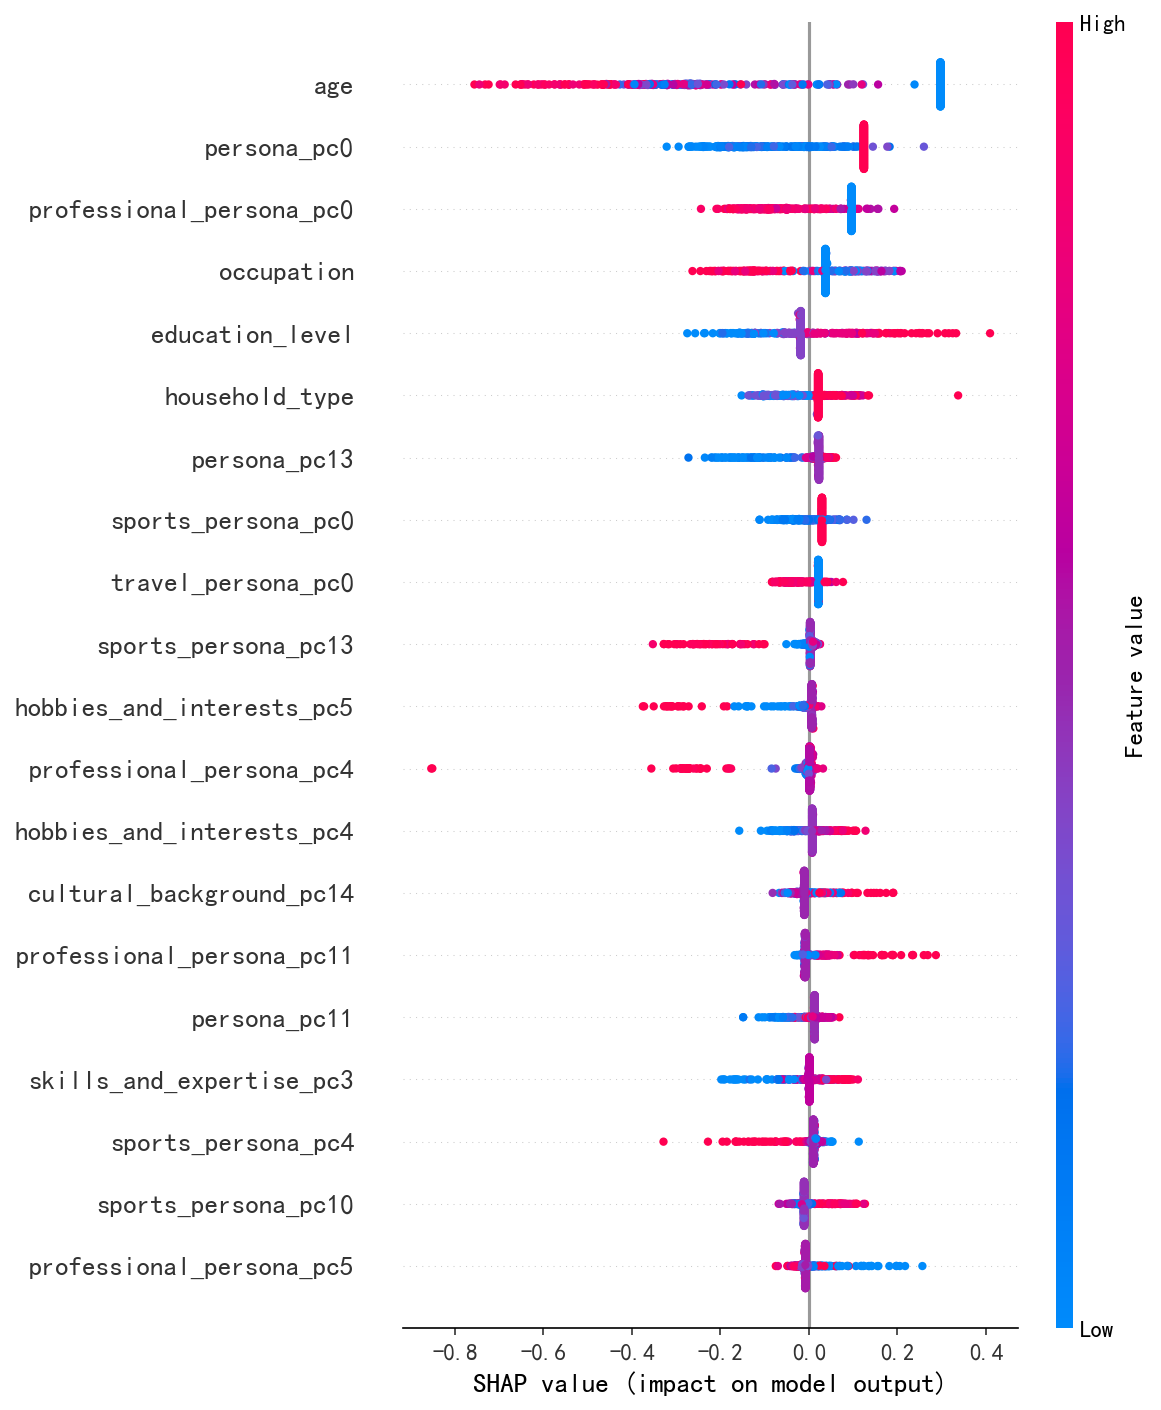
\includegraphics[width=\textwidth]{figures/shap_summary.png}
        \caption{SHAP summary plot}
        \label{fig:shap_summary}
    \end{subfigure}
    \hfill
    \begin{subfigure}{0.48\textwidth}
        \centering
        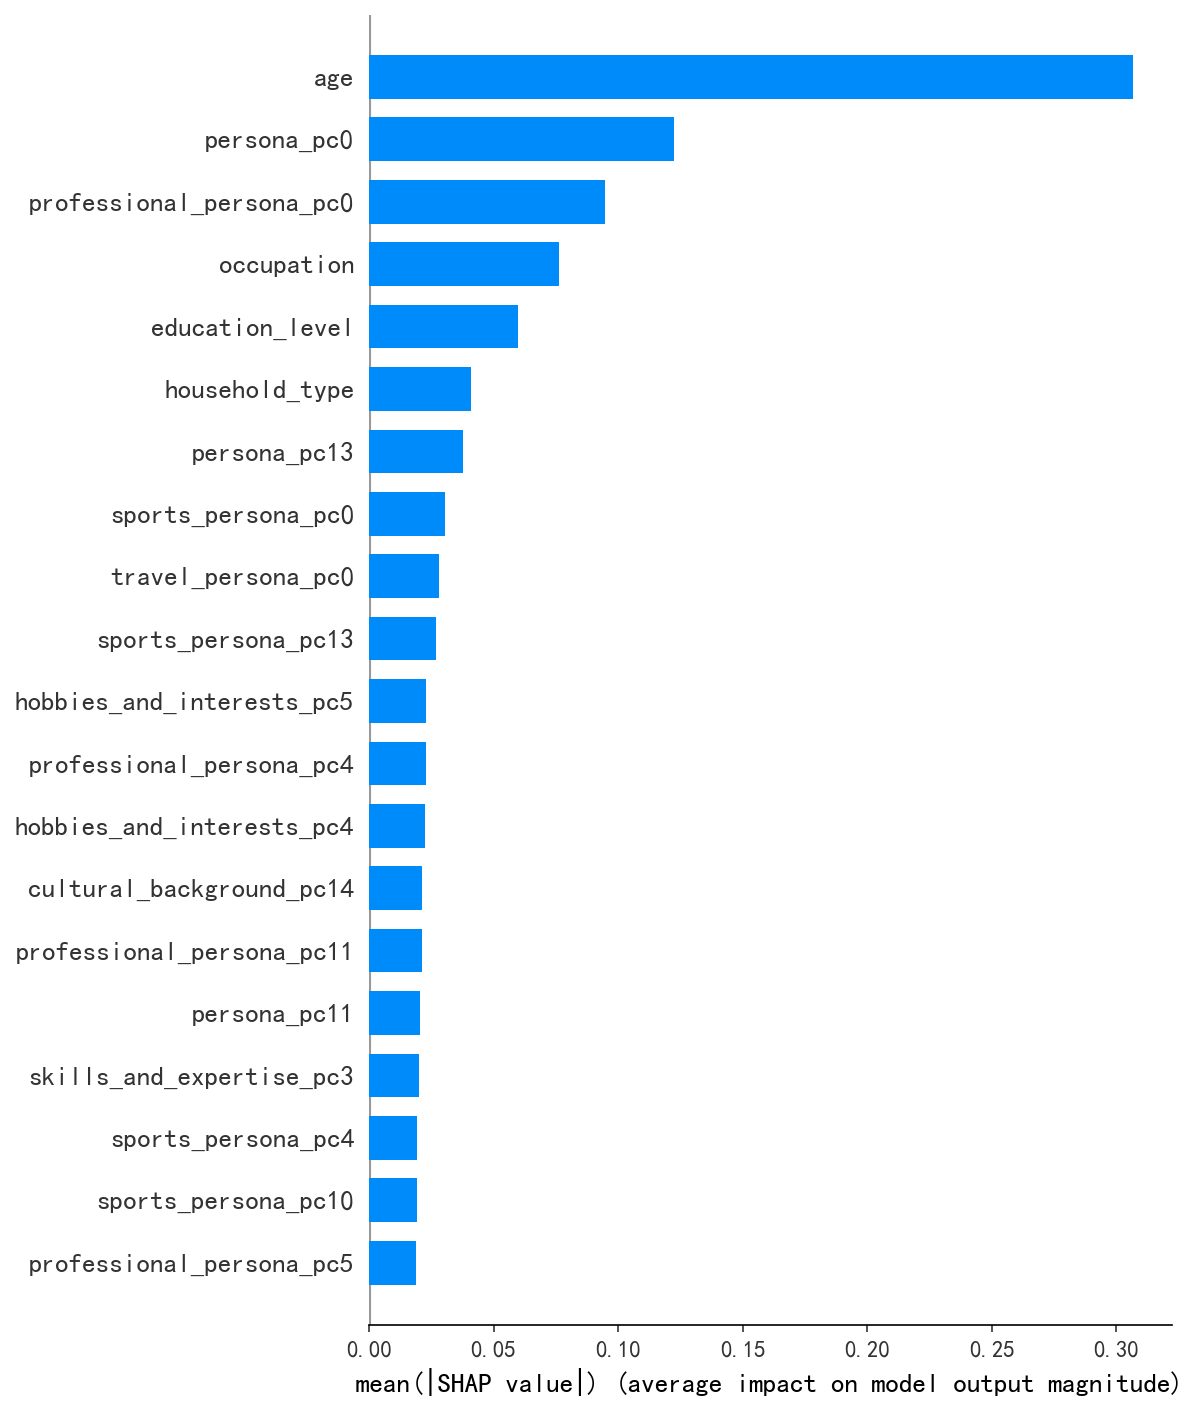
\includegraphics[width=\textwidth]{figures/shap_bar.png}
        \caption{SHAP bar chart}
        \label{fig:shap_bar}
    \end{subfigure}
    \caption{SHAP feature importance for the XGBoost regression model under Approach C (demographics + per-field PCA).}
    \label{fig:feature_importance}
\end{figure}

SHAP analysis reveals a starkly concentrated signal structure: \textbf{age} is by far the strongest predictor ($|$SHAP$|$=0.307$), dwarfing all other variables. This aligns tightly with the empirical reality of French retirement reform---changing the retirement age affects different age cohorts in fundamentally different ways: the calculus of a worker nearing retirement bears no resemblance to that of a recent university graduate. The second- and third-ranked features, persona\_pc0 ($|$SHAP$|$=0.122$) and professional\_persona\_pc0 ($|$SHAP$|$=0.095$), contribute only about one-third of age's magnitude, indicating that the overall semantic direction of personality and professional self-description carries modest attitude signal.

At the macro level, the 8 demographic features collectively account for 24\% of total SHAP magnitude, while the 160 text-derived PCA components account for 76\%. However, the text signal is highly dispersed---the average individual text PCA component contributes only $\sim$0.01 in $|$SHAP$|$, less than one-tenth of any single demographic feature. This dispersion explains why text embeddings fail to meaningfully improve R$^2$: although text fields collectively carry attitude-relevant information, the signal is scattered across many weak features and cannot coalesce into a predictive increment beyond a handful of strong demographic features. Among text fields, PCA components from persona (personality traits) and professional\_persona (career identity) appear most frequently in the Top-15, while lifestyle fields such as travel and culinary preferences rank lower. SHAP dependence plots (Appendix Figure~\ref{fig:shap_dependence}) confirm the negative relationship between age and predicted support score.

\subsection{The R$^2 \approx 0.28$ Ceiling}

The regression and classification results across all four feature sets (Tables~\ref{tab:regression_best} and~\ref{tab:classification_best}) converge on a single finding: \textbf{all roads lead to the same ceiling}.

\begin{table}[H]
    \centering
    \caption{Best regression model per approach (Test set)}
    \label{tab:regression_best}
    \begin{tabular}{@{}lcccc@{}}
        \toprule
        \textbf{Approach} & \textbf{Best Model} & \textbf{Test R$^2$} & \textbf{MAE} & \textbf{RMSE} \\
        \midrule
        D (+ global PCA) & Random Forest & 0.284 & 0.77 & 1.26 \\
        A (demographics only) & CatBoost & 0.273 & 0.76 & 1.27 \\
        B (+ persona\_text) & CatBoost & 0.272 & 0.77 & 1.27 \\
        C (+ per-field PCA) & CatBoost & 0.271 & 0.77 & 1.27 \\
        \bottomrule
    \end{tabular}
\end{table}

\begin{table}[H]
    \centering
    \caption{Best classification model per approach (Test set)}
    \label{tab:classification_best}
    \begin{tabular}{@{}lcccc@{}}
        \toprule
        \textbf{Approach} & \textbf{Best Model} & \textbf{Acc} & \textbf{Macro F1} \\
        \midrule
        A (demographics only) & Random Forest & 0.714 & 0.507 \\
        C (+ per-field PCA) & XGBoost & 0.704 & 0.504 \\
        B (+ persona\_text) & LightGBM & 0.723 & 0.489 \\
        D (+ global PCA) & Random Forest & 0.724 & 0.446 \\
        \bottomrule
    \end{tabular}
\end{table}

For regression, Test R$^2$ values are compressed within the narrow range of 0.271--0.284, with a maximum inter-approach difference of less than 0.015. Even the best-performing Approach D (R$^2$=0.284) improves over the demographics-only baseline (Approach A, R$^2$=0.273) by only $\sim$0.01---ten text fields, 3,840-dimensional SBERT embeddings, and carefully designed PCA dimensionality reduction collectively contribute roughly 1\% of additional explainable variance. Classification shows the same pattern: Macro F1 is concentrated between 0.446 and 0.507, with the demographics-only Approach A achieving the best result (0.507). Approach D performs worst in classification (0.446), suggesting that global PCA preserves continuous variance at the expense of discrete class separability.

Learning curves (Figure~\ref{fig:learning_curves}) provide further evidence: all four approaches converge after approximately 3,500 training samples, after which validation R$^2$ plateaus and additional data yields negligible gains. The persistent gap between train and validation R$^2$ confirms that the ceiling reflects a fundamental signal-to-noise limitation, not insufficient data.

\begin{figure}[H]
    \centering
    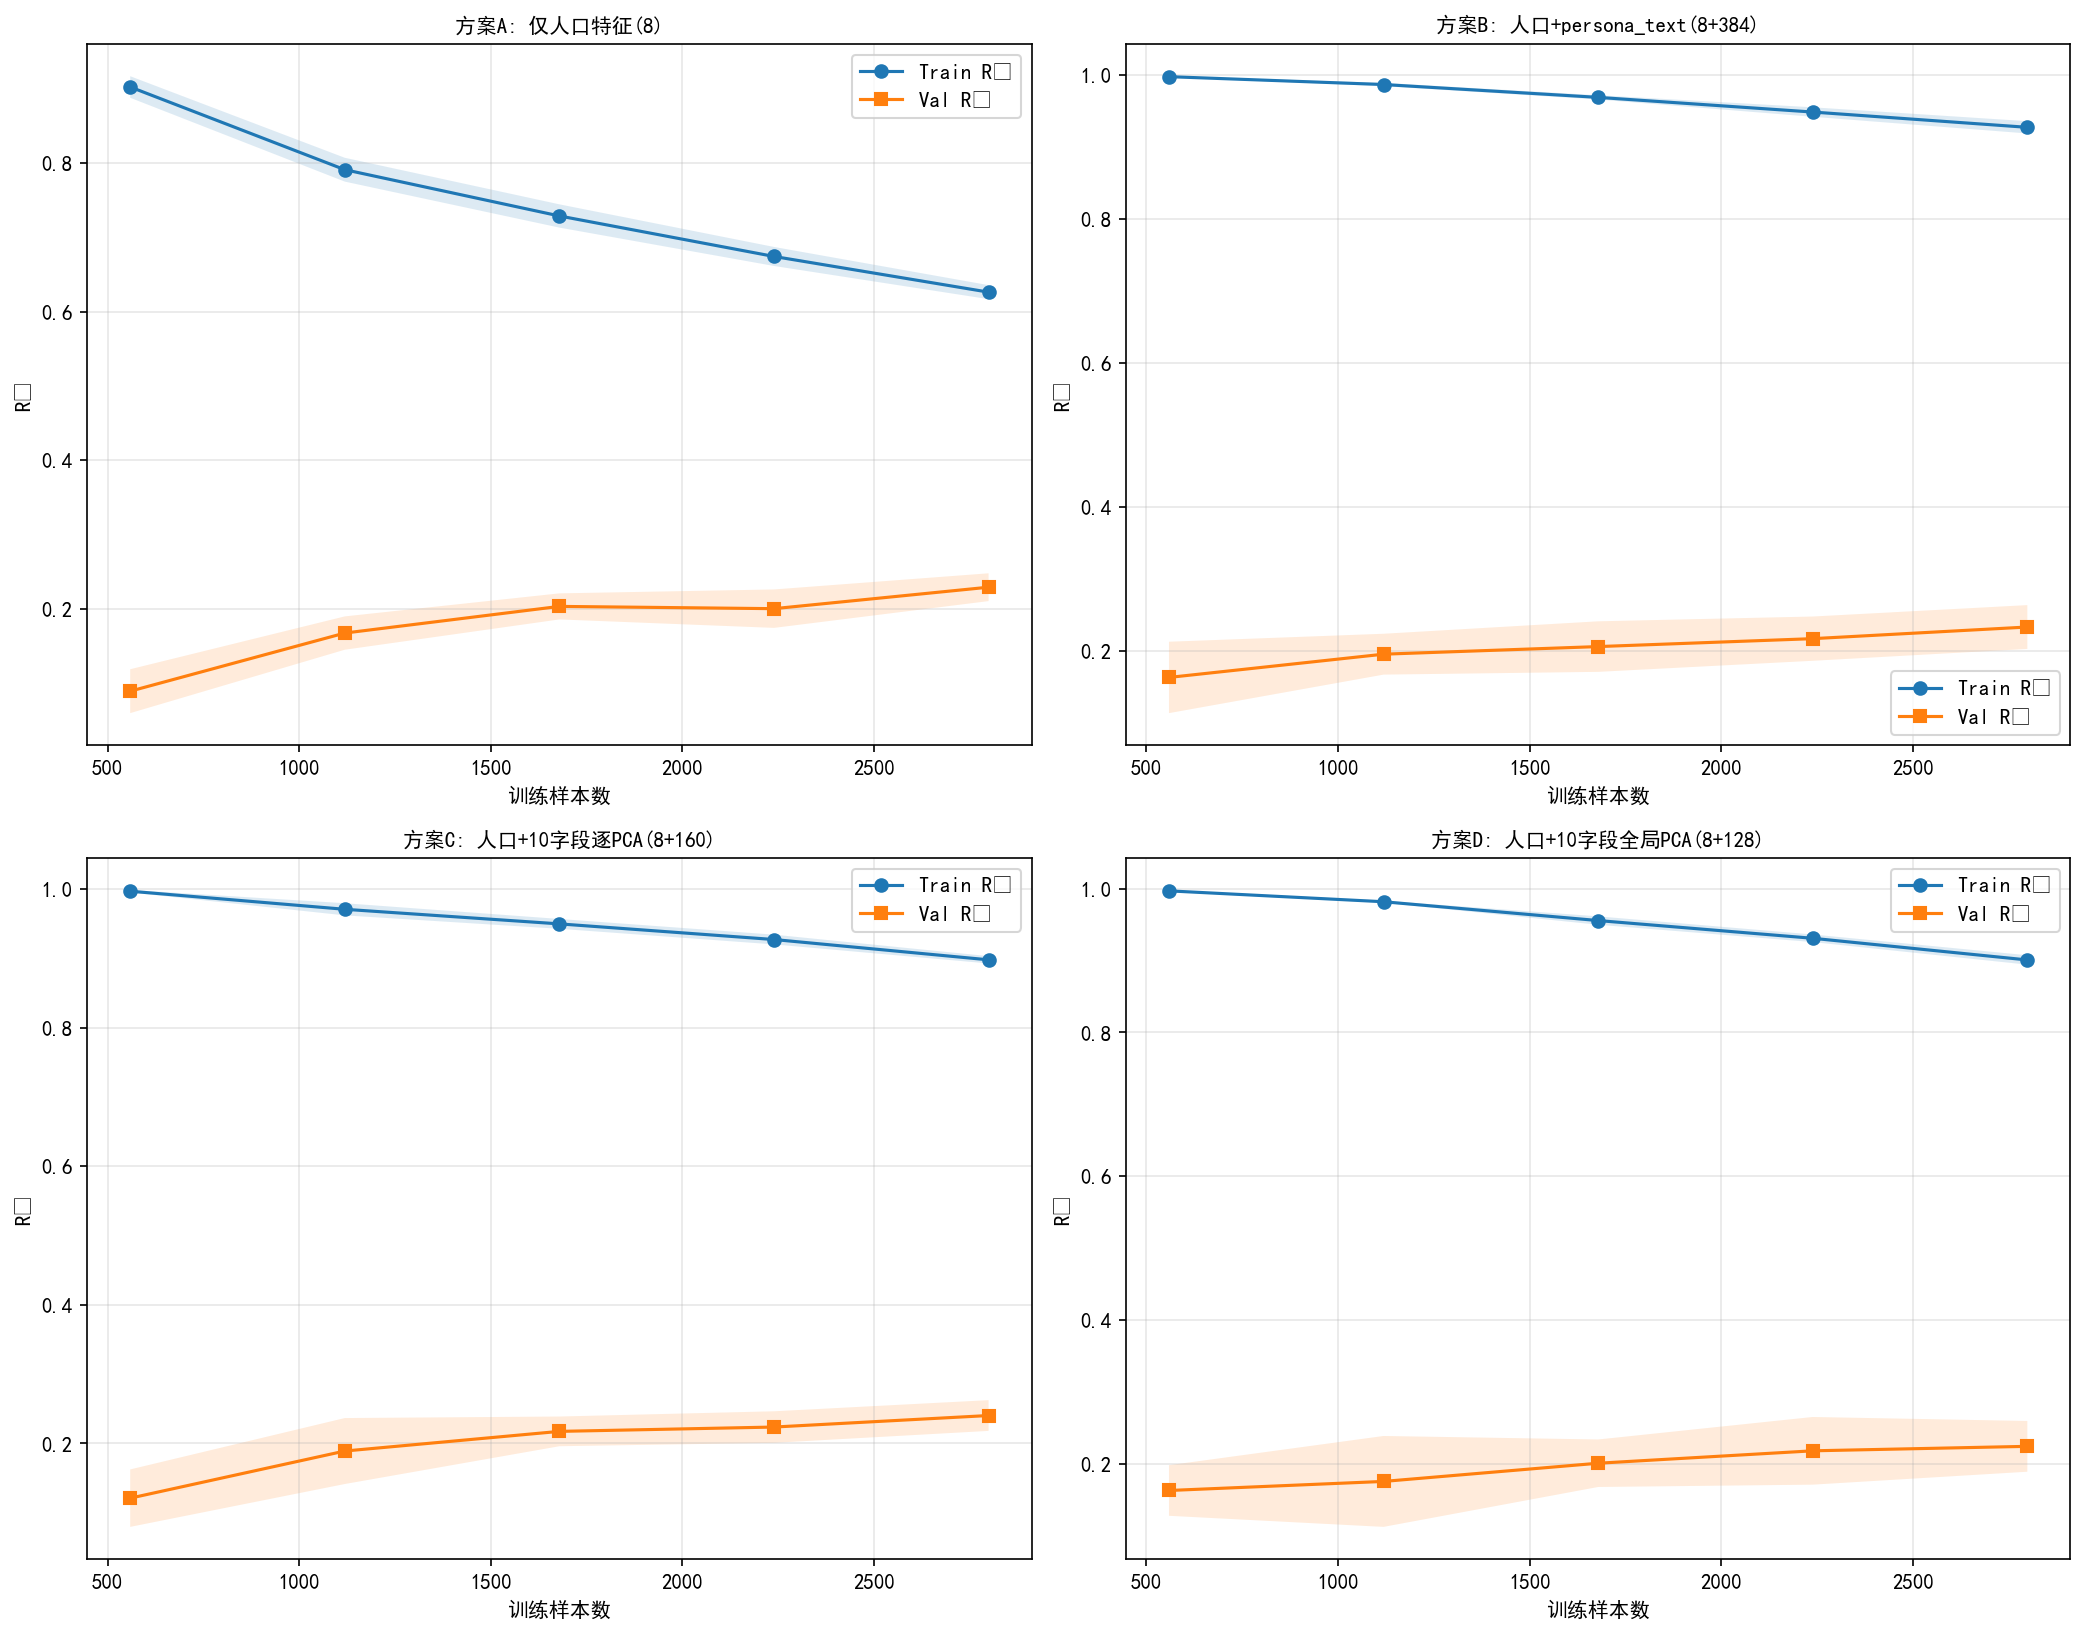
\includegraphics[width=0.95\textwidth]{figures/learning_curves.png}
    \caption{Learning curves across four feature construction approaches. All converge at similar validation R$^2$ levels.}
    \label{fig:learning_curves}
\end{figure}

Formally, decomposing the LLM support score as $y_i = f(x_i) + \epsilon_i$, where $f(x_i)$ represents the systematic persona--attitude relationship and $\epsilon_i$ is the LLM's sampling noise at $T=0.7$, our R$^2 \approx 0.28$ implies $\text{Var}(\epsilon) \approx 2.6 \times \text{Var}(f(x))$---\textbf{the LLM's random variation is roughly 2.6 times larger than the systematic variation from persona features}. Even if the same persona were queried repeatedly, the LLM would produce non-trivial variance in support scores due to sampling temperature, and this noise floor is insurmountable for any feature engineering strategy.

% ================================================================
\section{Discussion}
% ================================================================

\subsection{Prompt Sensitivity: Tool and Risk}

The most striking finding from the three-round prompt experiment---the 60-percentage-point swing in support---is both a powerful tool and a serious risk for LLM-based polling. \textbf{As a tool}, prompt engineering can substantially improve alignment with real benchmarks: Run 2's careful design choices (removing the neutrality prohibition, adding contextual awareness, retaining example anchoring) reduced the IFOP gap from +28pp to +12pp. \textbf{As a risk}, prompt sensitivity implies enormous researcher degrees of freedom---different wording choices can produce nearly arbitrary distributional outcomes. This demands that LLM polling studies fully report prompt designs and treat them as methodological variables subject to systematic testing, rather than implicit ``default settings.'' We recommend that future work adopt prompt ablation as a standard practice, just as traditional surveys report question wording and order effects.

\subsection{Redefining ``Representativeness''}

The similarity-versus-random comparison challenges an implicit assumption about representativeness in LLM polling. Traditional survey methodology pursues demographic representativeness, with random sampling as its gold standard. Yet our empirical results show that, in the LLM simulation context, random sampling produces a distribution that deviates \textit{more} from the real benchmark. The root cause is that LLM role-playing does not perform uniformly across all personas---when a persona lacks semantic connection to the issue, the LLM's ``role-play'' degrades into ``guessing,'' and its responses no longer reflect any systematic relationship between persona features and attitudes. In this scenario, demographic ``representativeness'' amounts to averaging over a large number of irrelevant responses, diluting meaningful attitude signals.

We therefore argue that ``representativeness'' in LLM polling should encompass at least two dimensions: demographic balance \textit{and} semantic relevance. Similarity-based retrieval should not be dismissed as a ``bias'' to eliminate, but recognized as an active sample design strategy, methodologically isomorphic to screening questions in traditional surveys and participant selection in quasi-experiments. The critical requirement is that researchers explicitly report their sampling strategy and its implications for the scope of conclusions.

\subsection{The Fundamental Limit of Individual Prediction}

The convergence of all feature sets and models to the same R$^2$ ceiling ($\approx$0.28) shifts the question from ``which approach is better?'' to ``why does a ceiling exist?'' Our analysis points to the irreducible noise introduced by LLM sampling temperature: at $T=0.7$, repeated queries of the same persona exhibit substantial variance uncorrelated with any observable feature. In classification, even with balanced class weights, the Macro F1 ceiling ($\approx$0.51) remains far from practically usable accuracy. This means that reliable individual-level political stance prediction from LLM-generated data is not yet feasible under the current paradigm. Lower temperatures, repeated sampling with averaging, or larger models may partially mitigate this issue, but the fundamental stochasticity of LLM decoding is unlikely to be fully eliminated.

\subsection{Limitations}

Our study has several limitations. First, we tested only one policy topic (retirement reform) and one LLM (DeepSeek-V4-Flash); results may differ for other topics or models. Second, the 10,000-sample size, while sufficient for ML modeling, limits the statistical power of demographic subgroup analysis. Third, the IFOP benchmark (n=2,023) has its own sampling error, so the ``ground truth'' is uncertain. Fourth, we did not systematically vary sampling temperature or measure test-retest reliability, which would directly quantify the LLM noise floor. Fifth, all prompts were in Chinese with French persona contexts, potentially introducing language-conditioning effects.

% ================================================================
\section{Conclusion}
% ================================================================

This paper presents a systematic empirical investigation of LLM behavioral patterns in simulating French citizens' attitudes toward retirement reform. Through three prompt ablation rounds, two sampling strategies, and comprehensive ML modeling, we arrive at three main conclusions:

(1) \textbf{Prompt design exerts decisive influence on LLM attitude simulation.} Prompt wording changes alone produced a 60-percentage-point support-rate swing across iterations---an effect size exceeding that of real-world social movements. Run 2's careful design reduced the IFOP gap to +12pp, demonstrating the methodological viability of prompt engineering.

(2) \textbf{Sampling strategy significantly affects simulation quality, and semantic filtering outperforms random sampling.} By focusing on an issue-relevant subpopulation, similarity-based retrieval achieved aggregate distributions closer to real benchmarks than random sampling. This counterintuitive finding indicates that ``representativeness'' in LLM polling should not be equated with demographic balance; semantic relevance is at least equally important.

(3) \textbf{Individual-level attitude prediction faces a hard performance ceiling.} Age is the only substantively predictive feature ($|$SHAP$|$=0.307$), with text embeddings providing negligible additional predictive power. All feature sets and models converge to R$^2 \approx 0.28$, constrained by irreducible LLM sampling noise. This finding sets an empirical boundary for applications that require individual-level political analysis from LLM-generated data.

Future work includes extending the framework to additional policy topics for cross-issue generalization, systematically varying LLM temperature to quantify the stochasticity--noise relationship, incorporating real survey microdata for direct individual-level validation, and exploring politically fine-tuned attitude encoders as alternatives to generic Sentence-BERT embeddings.

\section*{Acknowledgments}
We thank IFOP, ELABE, and Odoxa for making their survey data publicly available, and SiliconFlow for providing API access to DeepSeek-V4-Flash.

% ── References ─────────────────────────────────────────────────
\begin{thebibliography}{20}

\bibitem{groves2009survey}
R.~M. Groves, F.~J. Fowler, M.~P. Couper, J.~M. Lepkowski, E.~Singer, and R.~Tourangeau.
\newblock \textit{Survey Methodology}, 2nd ed. Wiley, 2009.

\bibitem{argyle2023out}
L.~P. Argyle, E.~C. Busby, N.~Fulda, J.~R. Gubler, C.~Rytting, and D.~Wingate.
\newblock Out of one, many: Using language models to simulate human samples.
\newblock \textit{Political Analysis}, 31(3):337--351, 2023.

\bibitem{santurkar2023whose}
S.~Santurkar, E.~Durmaz, F.~Ladhak, C.~Lee, P.~Liang, and T.~Hashimoto.
\newblock Whose opinions do language models reflect?
\newblock In \textit{ICML}, 2023.

\bibitem{park2023generative}
J.~S. Park, J.~C. O'Brien, C.~J. Cai, M.~R. Morris, P.~Liang, and M.~S. Bernstein.
\newblock Generative agents: Interactive simulacra of human behavior.
\newblock In \textit{UIST}, 2023.

\bibitem{barbera2015tweeting}
P.~Barber\'a.
\newblock Birds of the same feather tweet together: Bayesian ideal point estimation using Twitter data.
\newblock \textit{Political Analysis}, 23(1):76--91, 2015.

\bibitem{hersh2015hacking}
E.~D. Hersh.
\newblock \textit{Hacking the Electorate: How Campaigns Perceive Voters}. Cambridge University Press, 2015.

\bibitem{montgomery2018predicting}
J.~M. Montgomery and S.~Olivella.
\newblock Predicting elections with big data.
\newblock In \textit{The Oxford Handbook of Electoral Systems}, 2018.

\bibitem{reimers2019sentence}
N.~Reimers and I.~Gurevych.
\newblock Sentence-BERT: Sentence embeddings using Siamese BERT-networks.
\newblock In \textit{EMNLP-IJCNLP}, 2019.

\bibitem{ifop2025retraites}
IFOP/CGT.
\newblock Les Fran\c{c}ais et la r\'eforme des retraites.
\newblock Technical report, April 2025.

\bibitem{elabe2026}
ELABE/BFMTV.
\newblock L'\'etat d'esprit des Fran\c{c}ais pour 2026.
\newblock Technical report, January 2026.

\end{thebibliography}

% ── Appendix ───────────────────────────────────────────────────
\appendix
\section{Full Regression Results}

\begin{table}[H]
    \centering
    \caption{All regression models $\times$ all approaches (Val set, sorted by R$^2$)}
    \label{tab:regression_all}
    \resizebox{\textwidth}{!}{%
    \begin{tabular}{@{}llrrr@{}}
        \toprule
        \textbf{Approach} & \textbf{Model} & \textbf{Val R$^2$} & \textbf{Val MAE} & \textbf{5-Fold CV R$^2$} \\
        \midrule
        D & Random Forest & 0.276 & 0.79 & 0.253 $\pm$ 0.036 \\
        C & CatBoost & 0.275 & 0.79 & 0.259 $\pm$ 0.035 \\
        D & CatBoost & 0.271 & 0.79 & 0.256 $\pm$ 0.033 \\
        C & Random Forest & 0.273 & 0.79 & 0.253 $\pm$ 0.034 \\
        B & CatBoost & 0.258 & 0.80 & 0.247 $\pm$ 0.027 \\
        A & CatBoost & 0.252 & 0.79 & 0.258 $\pm$ 0.021 \\
        \bottomrule
    \end{tabular}%
    }
\end{table}

\section{Prompt Templates}

\textbf{Run 2 (Best-Performing) Prompt:}

\begin{quote}
\small
你是一位法国公民，请根据人物画像回答政策问题。

【基础信息】/【社会背景】/【个人画像】/【兴趣爱好】/【职业发展】
\textit{[persona details inserted here]}

【问题】关于法定退休年龄，您认为应该怎么做？回到62岁、维持在64岁，还是进一步提高？

【要求】
1. 第一人称"我"视角
2. 用中文，简短精炼准确
3. 结合自身画像，真实自然
4. 请结合你对当前法国形势的理解，更真实地扮演角色，摒弃你自身内置的价值观，回答需具有实时性
5. 避免过度极端语气，理性客观
6. 结尾标注：支持度：X/10（0-10分）

示例：作为一名45岁男性工人，我认为...支持度：3/10
\end{quote}

\section{Reproducibility}

All code is available in the project repository at \texttt{french\_policy\_simulator/}. The main analysis pipeline can be executed via:

\begin{verbatim}
python scripts/05_ml_modeling.py
\end{verbatim}

Configuration parameters (RANDOM\_STATE=42, TRAIN\_SIZE=0.70, VAL\_SIZE=0.15, PCA\_DIMS\_PER\_FIELD=16, PCA\_DIMS\_GLOBAL=128) are specified at the top of the script. The Sentence-BERT model (\texttt{all-MiniLM-L6-v2}) is cached locally for offline use.

\section{Supplementary Figures}

\begin{figure}[H]
    \centering
    \begin{subfigure}{0.48\textwidth}
        \centering
        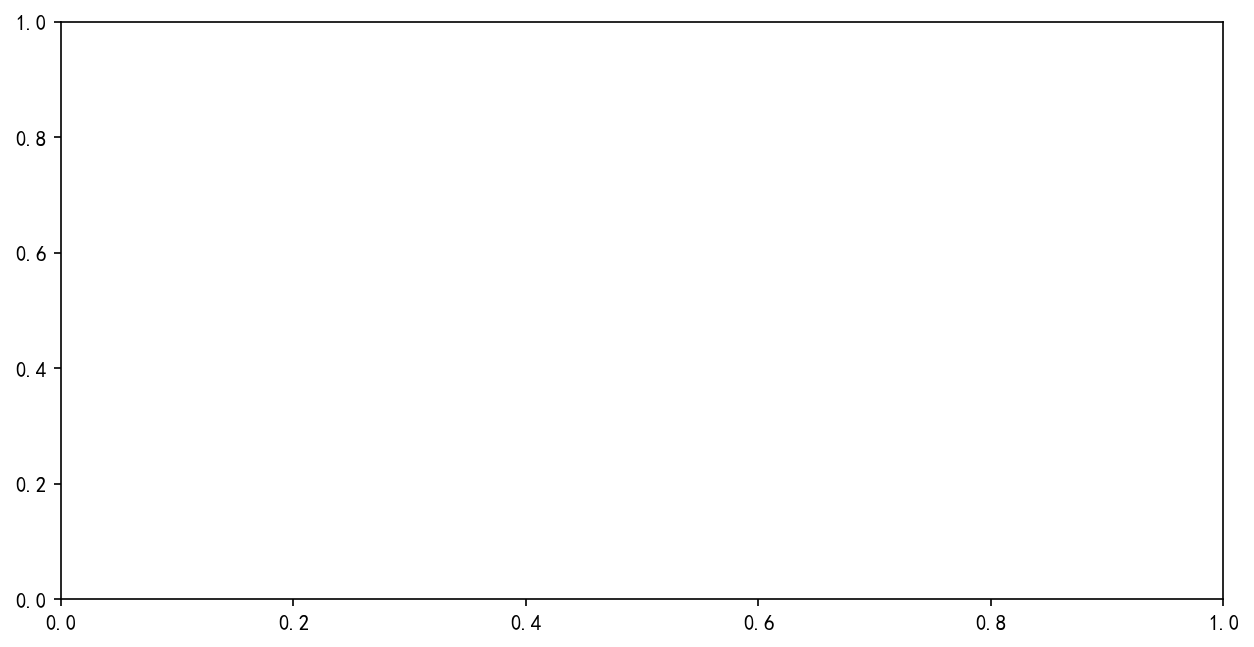
\includegraphics[width=\textwidth]{figures/shap_dependence_1.png}
        \caption{SHAP dependence: age vs.\ predicted value}
    \end{subfigure}
    \hfill
    \begin{subfigure}{0.48\textwidth}
        \centering
        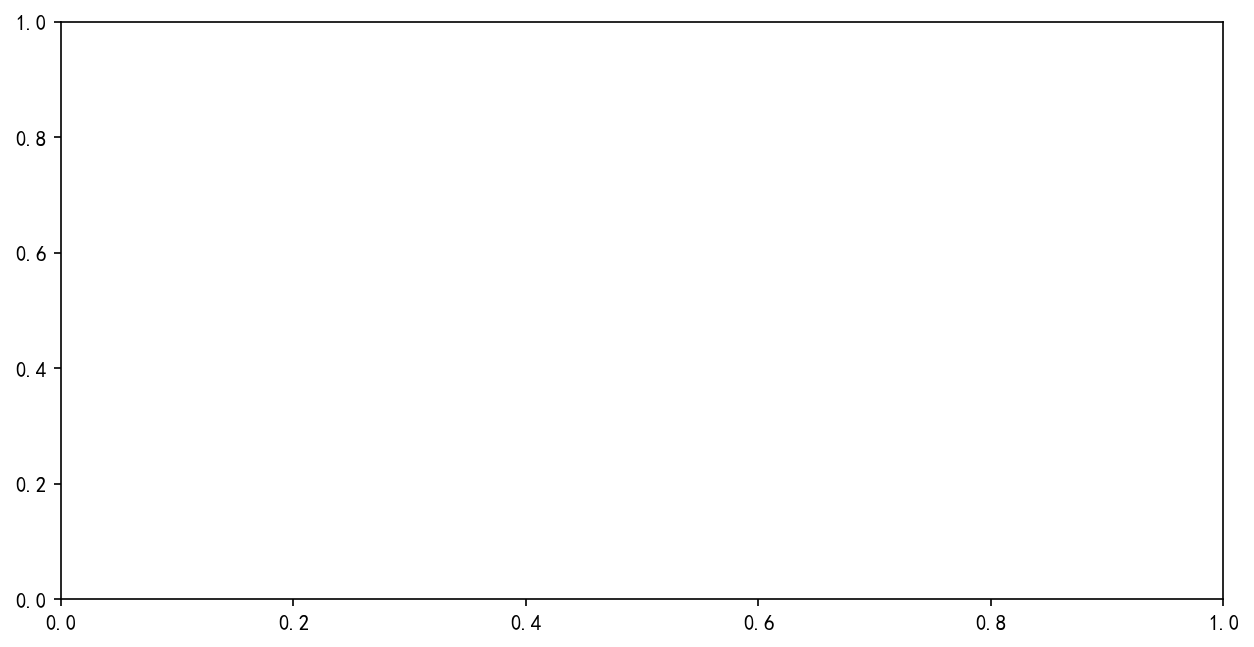
\includegraphics[width=\textwidth]{figures/shap_dependence_2.png}
        \caption{SHAP dependence: persona\_pc0 vs.\ predicted value}
    \end{subfigure}
    \caption{SHAP dependence plots for the top two features. Age shows a clear negative relationship with predicted support score.}
    \label{fig:shap_dependence}
\end{figure}

\begin{figure}[H]
    \centering
    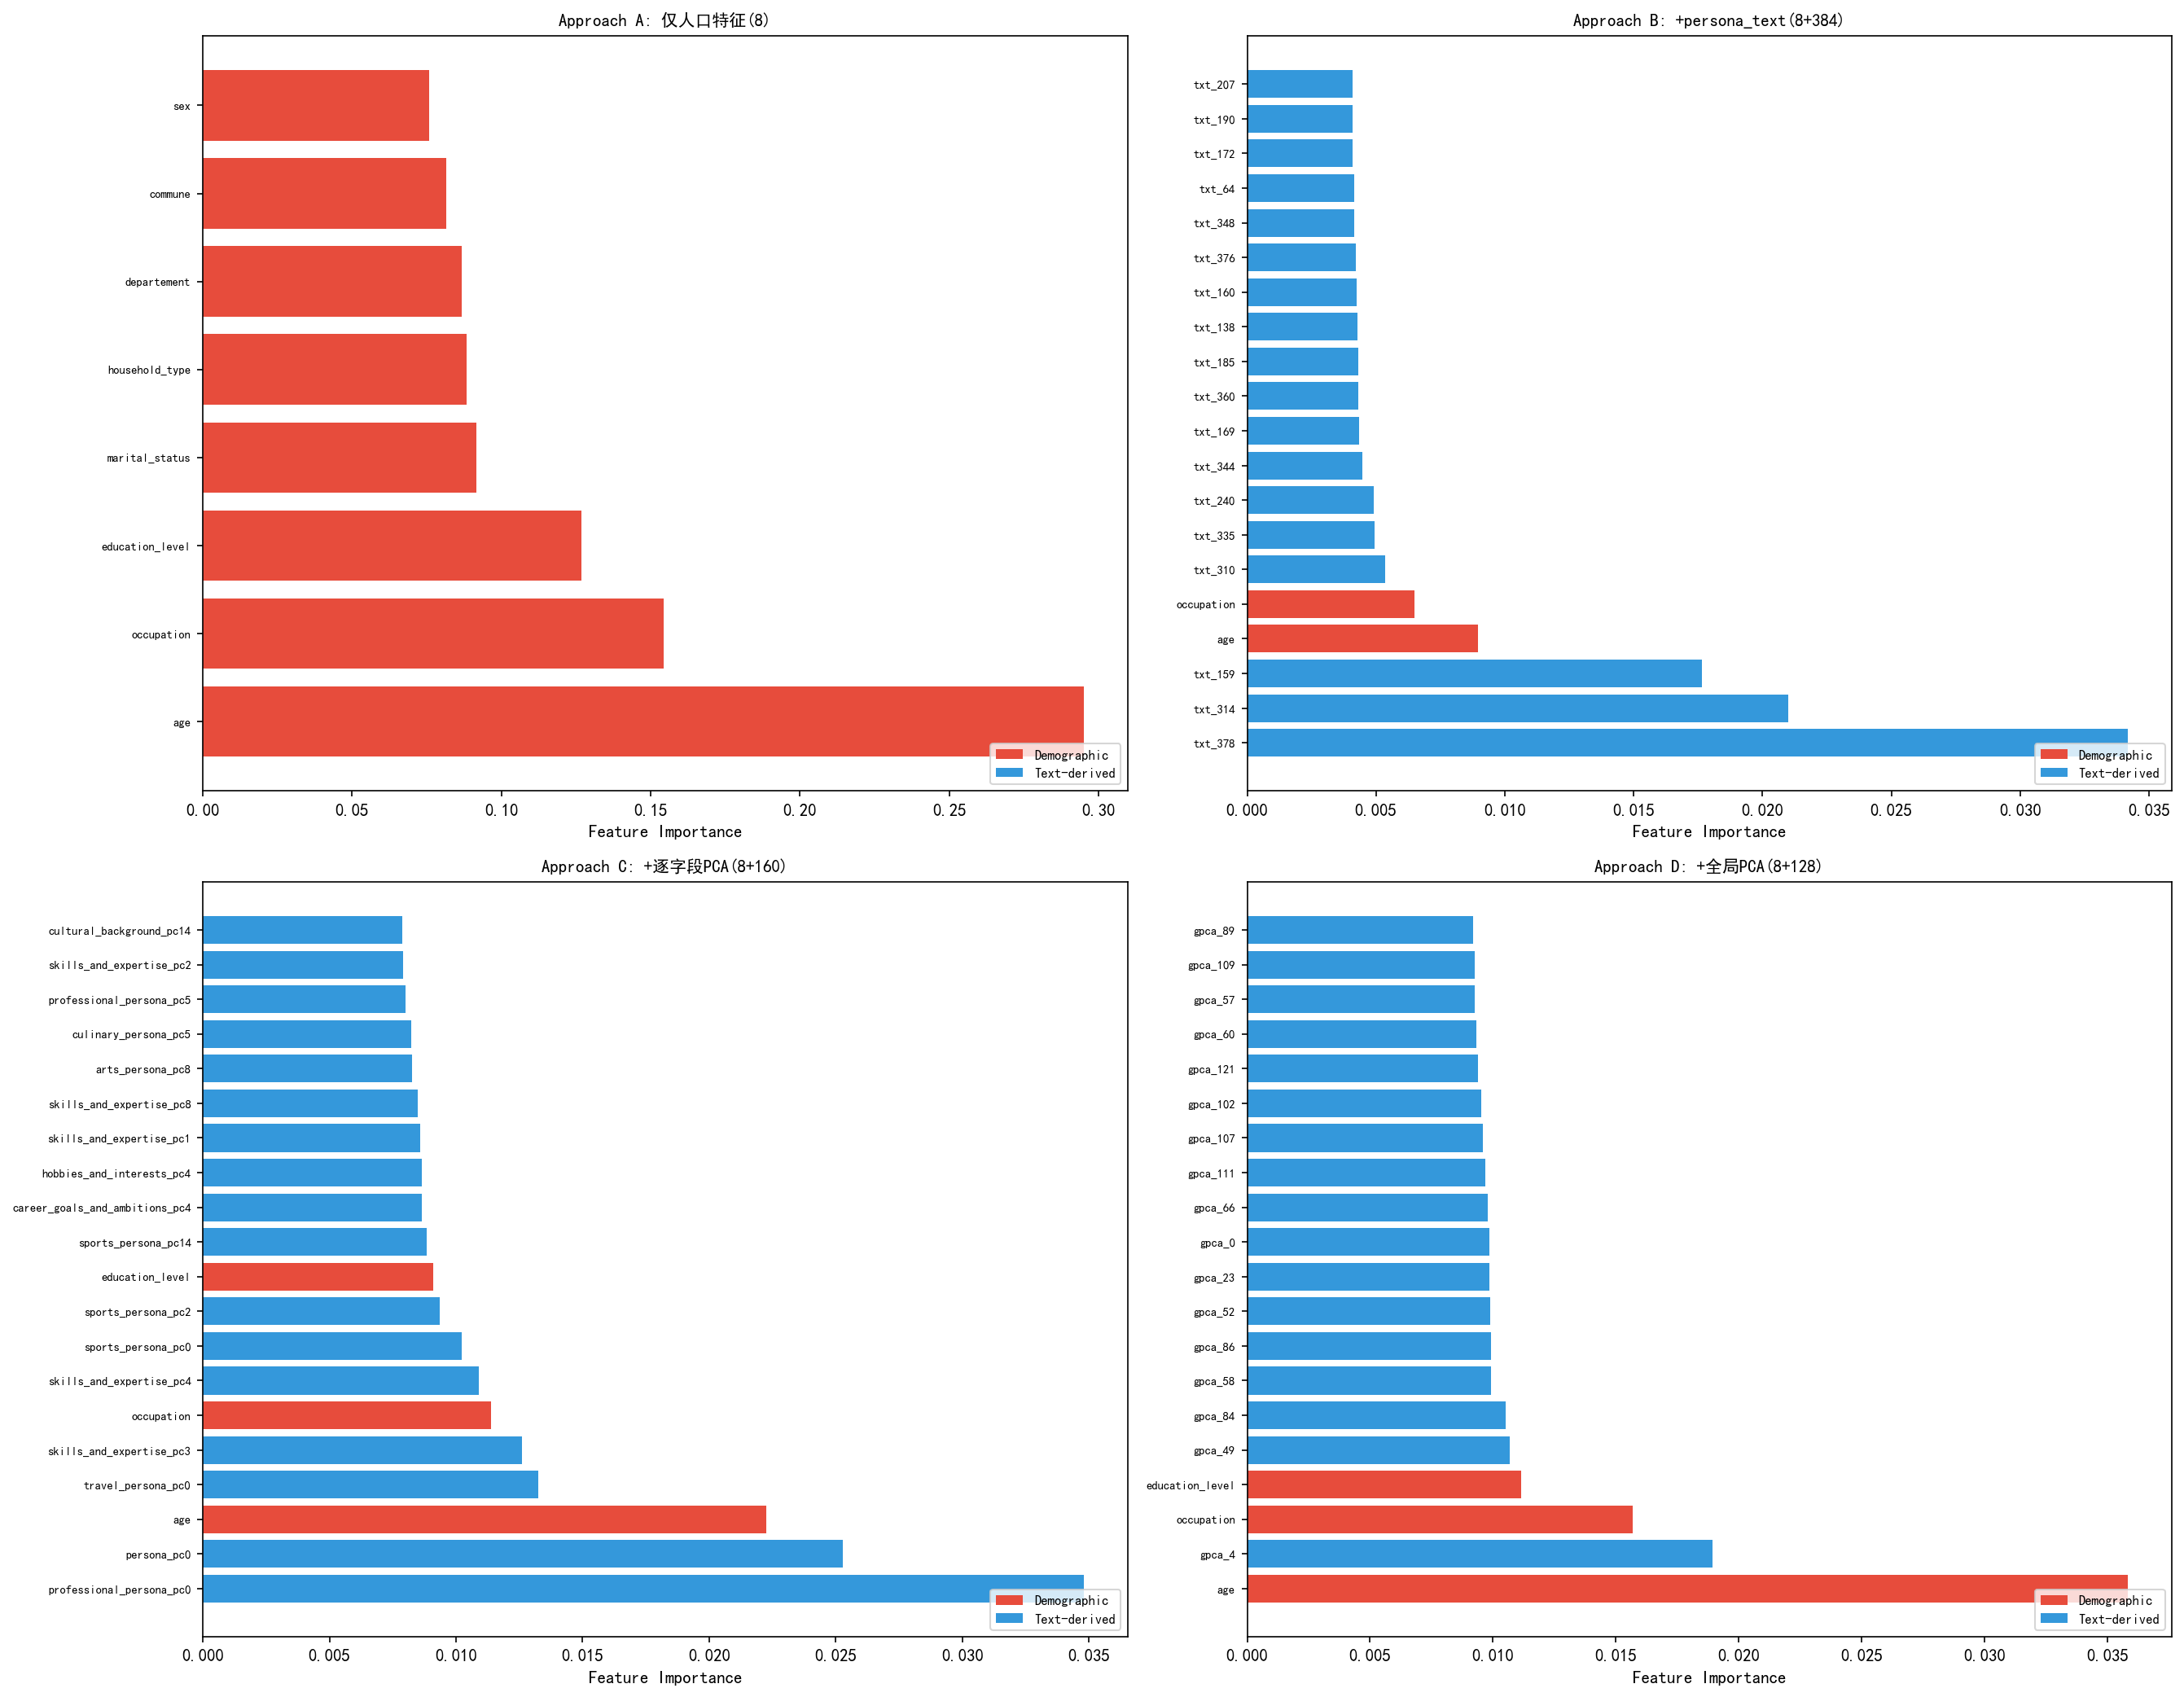
\includegraphics[width=0.95\textwidth]{figures/feature_importance_grid.png}
    \caption{XGBoost feature importance Top-20 across the four approaches.}
    \label{fig:feature_importance_grid}
\end{figure}

\begin{figure}[H]
    \centering
    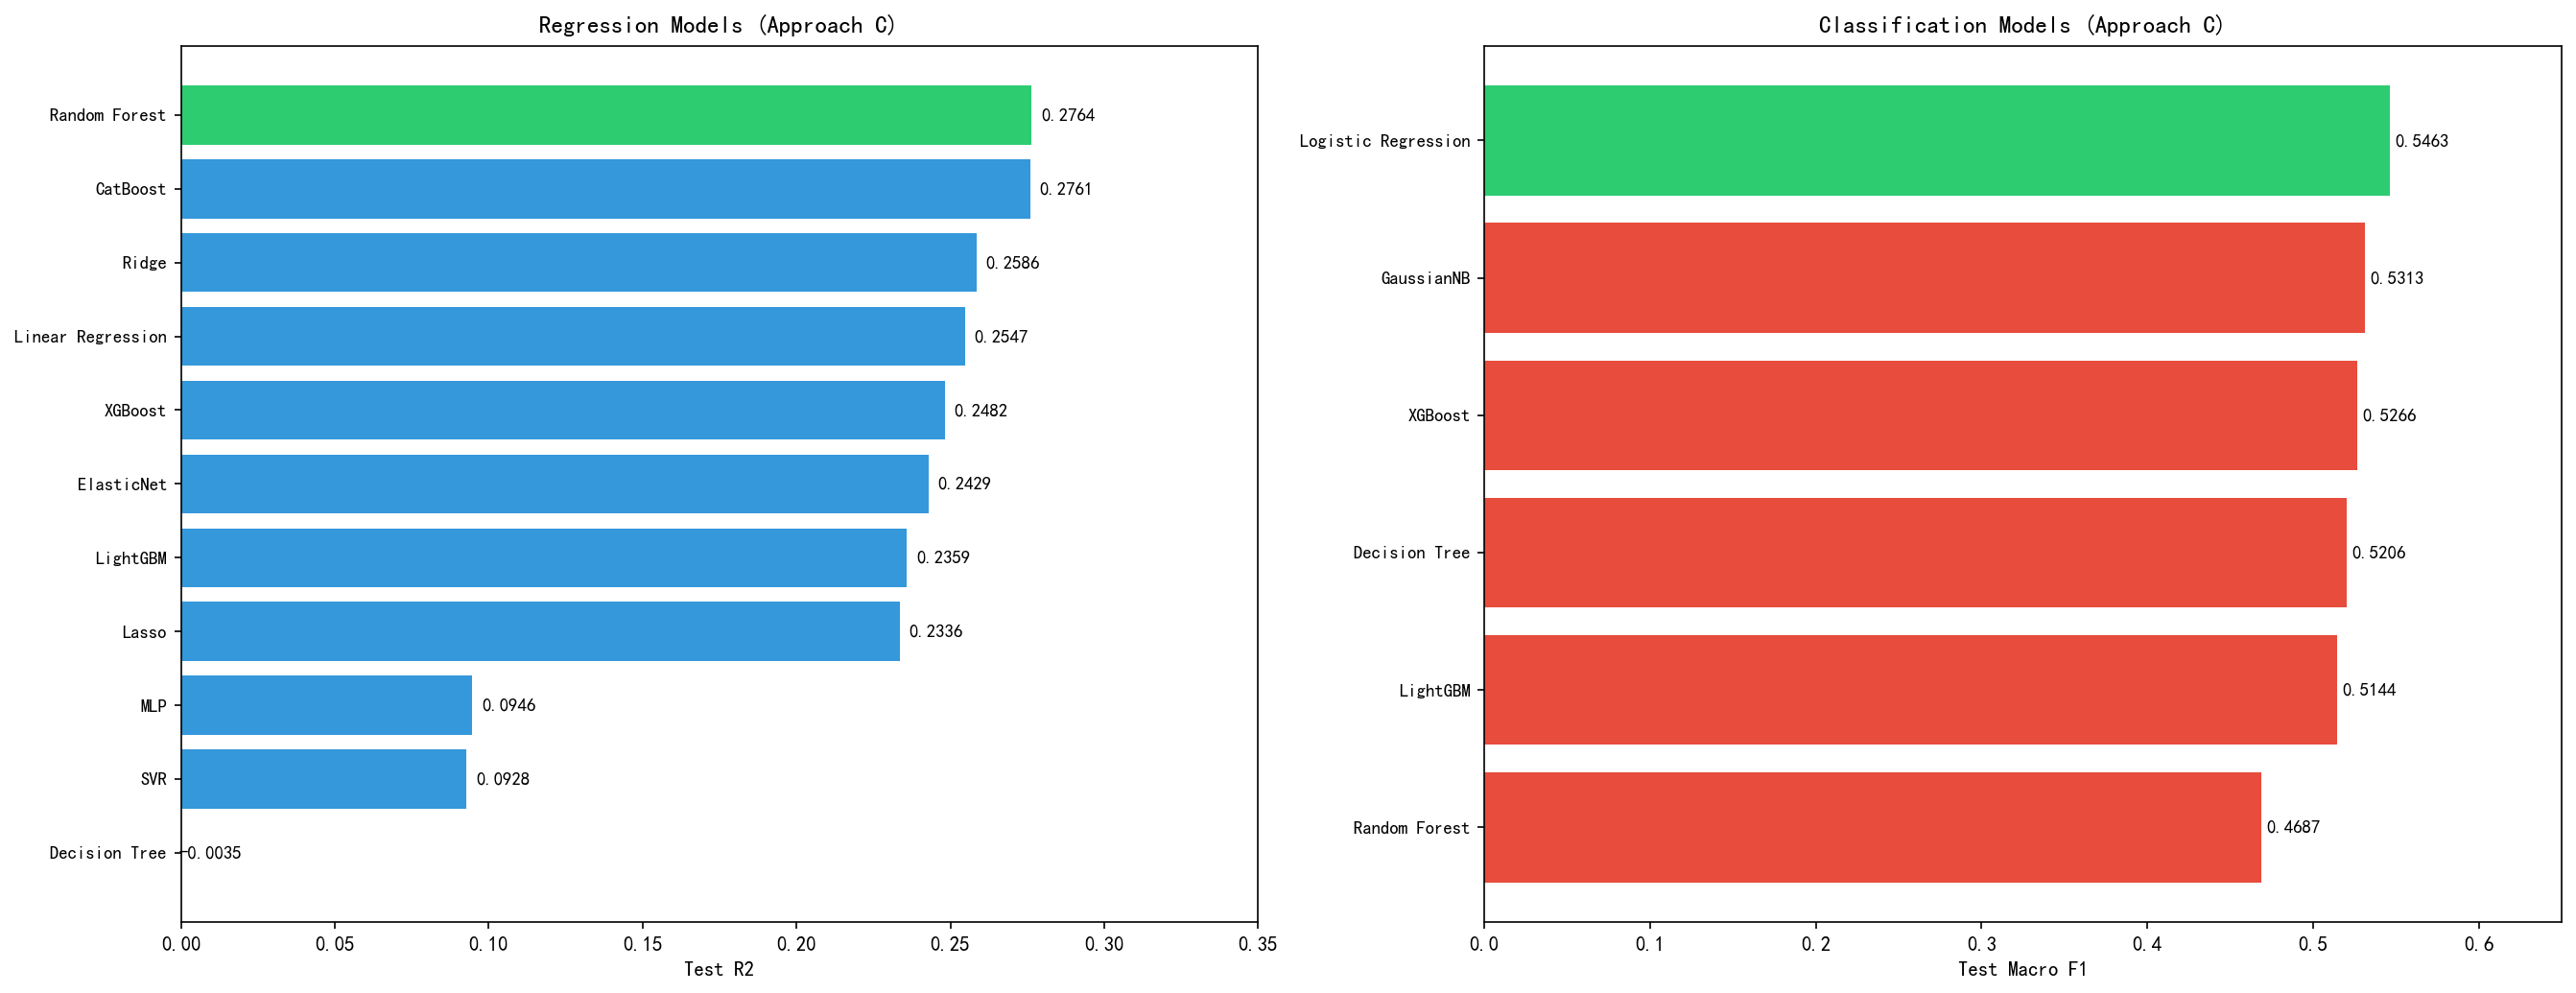
\includegraphics[width=0.95\textwidth]{figures/model_comparison.png}
    \caption{Test-set performance comparison of all regression (left) and classification (right) models under Approach C.}
    \label{fig:model_comparison}
\end{figure}

\begin{figure}[H]
    \centering
    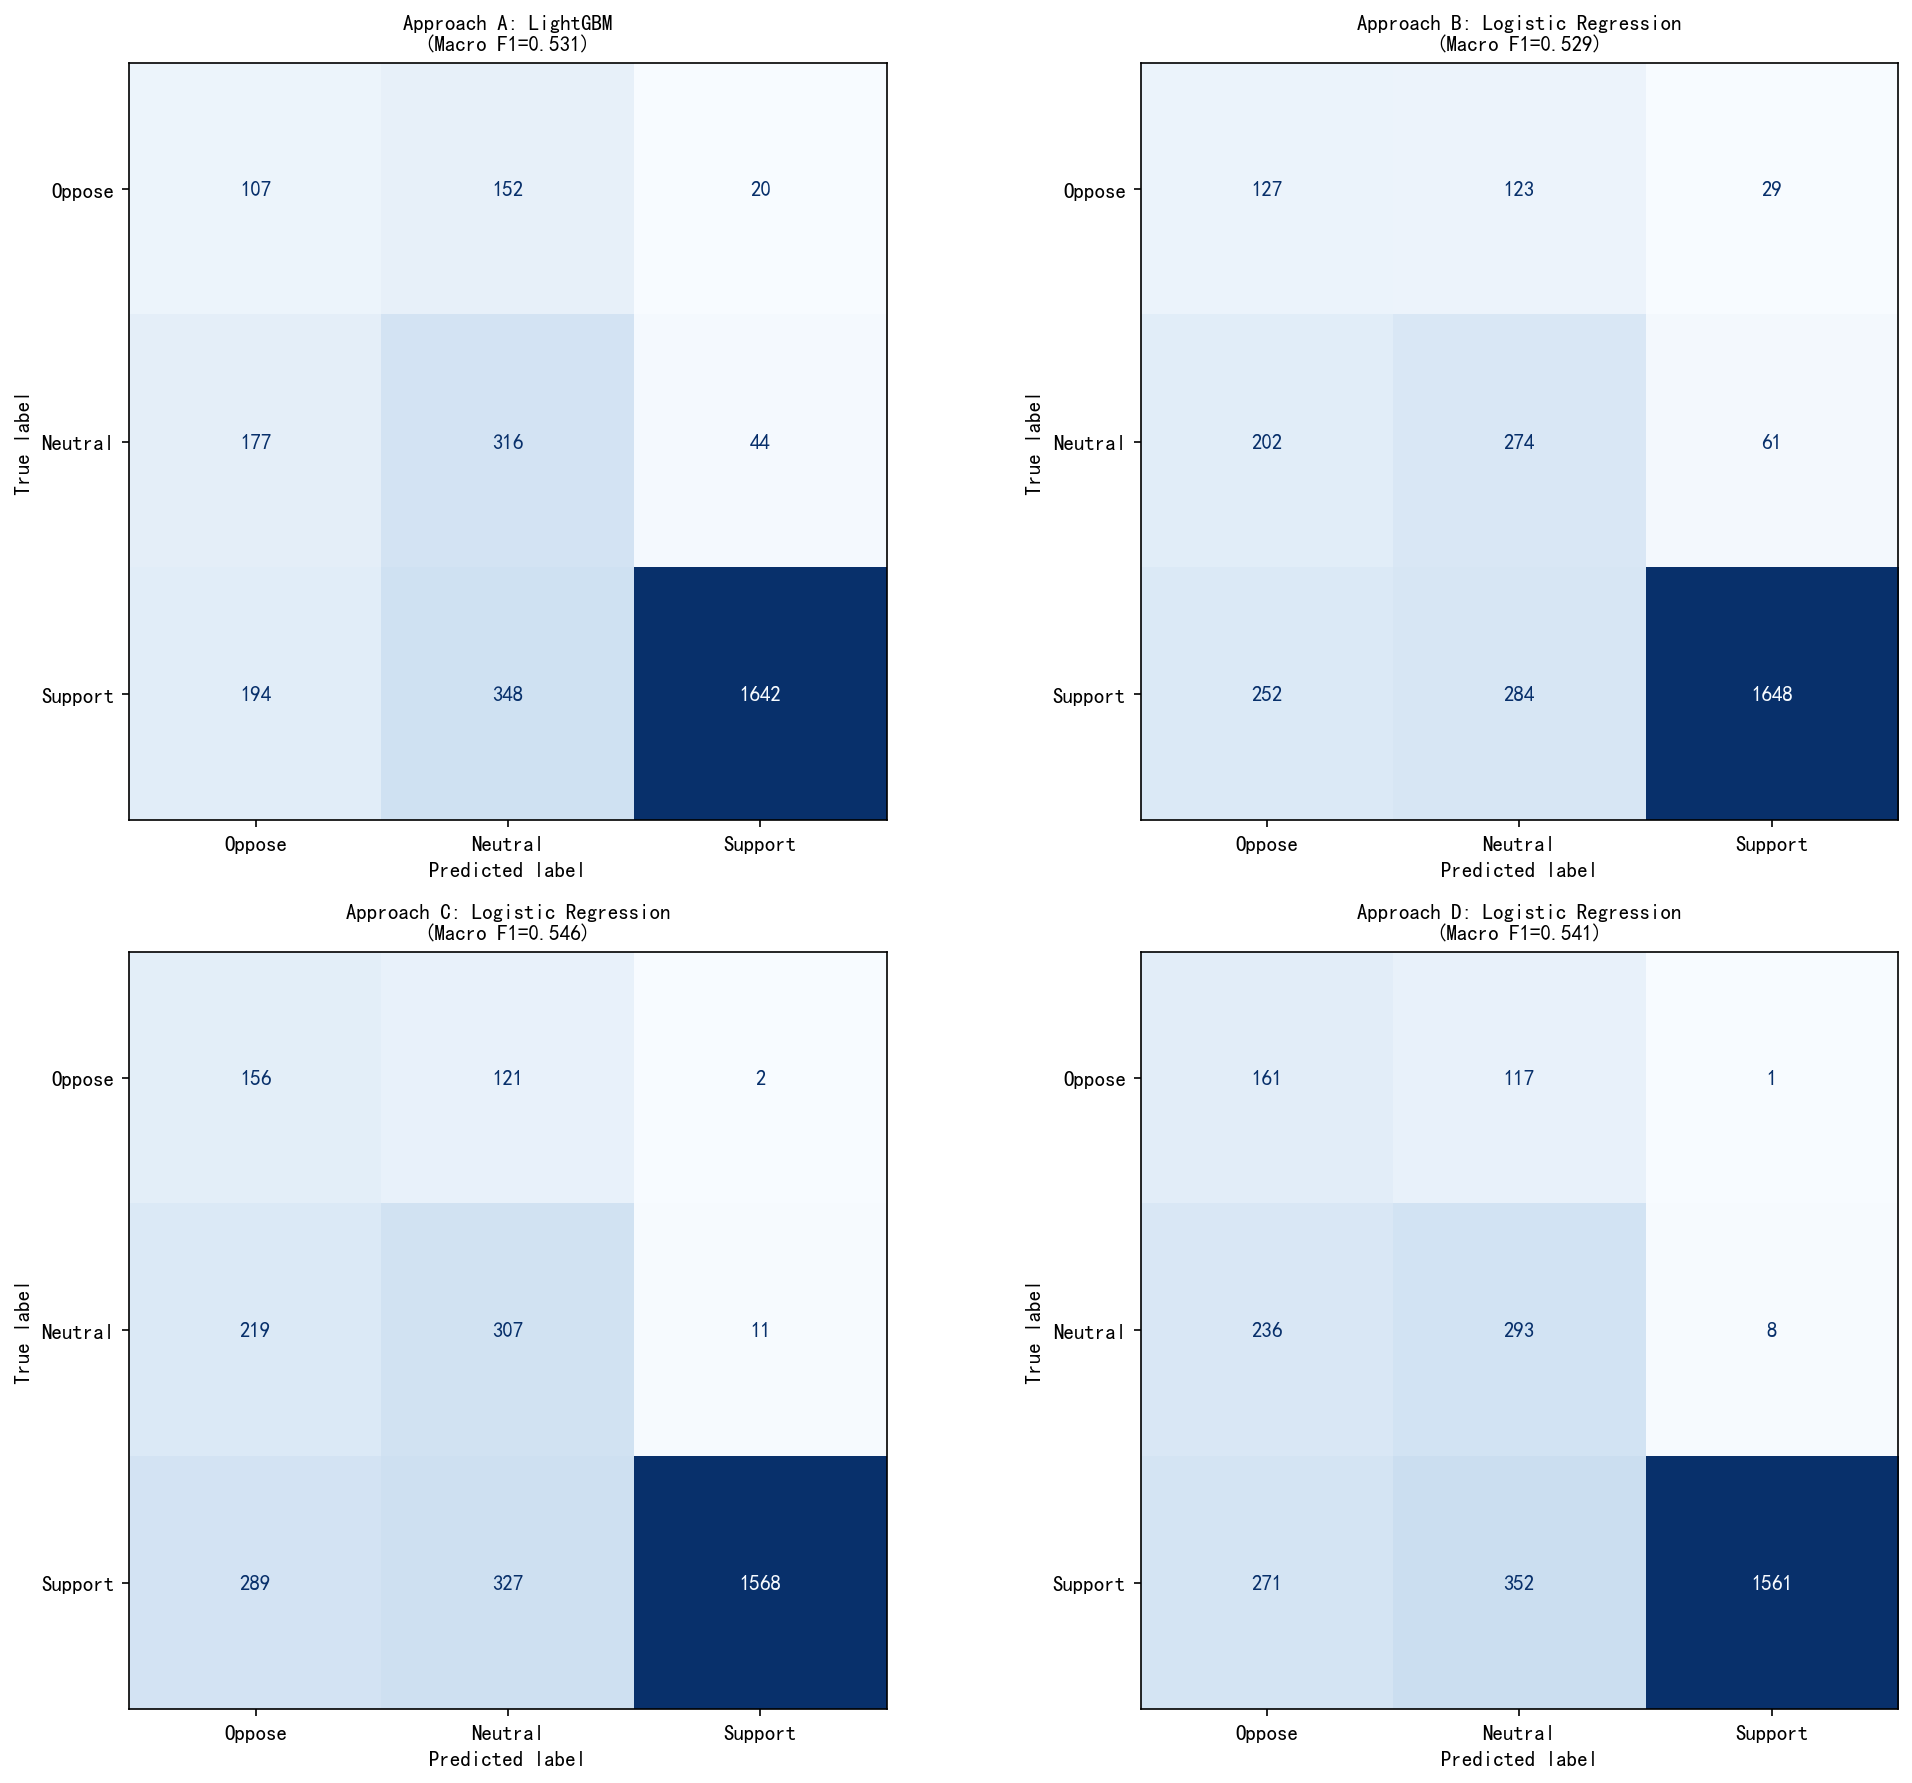
\includegraphics[width=0.95\textwidth]{figures/confusion_matrices.png}
    \caption{Confusion matrices for the best classifier under each approach.}
    \label{fig:confusion_matrices}
\end{figure}

\begin{figure}[H]
    \centering
    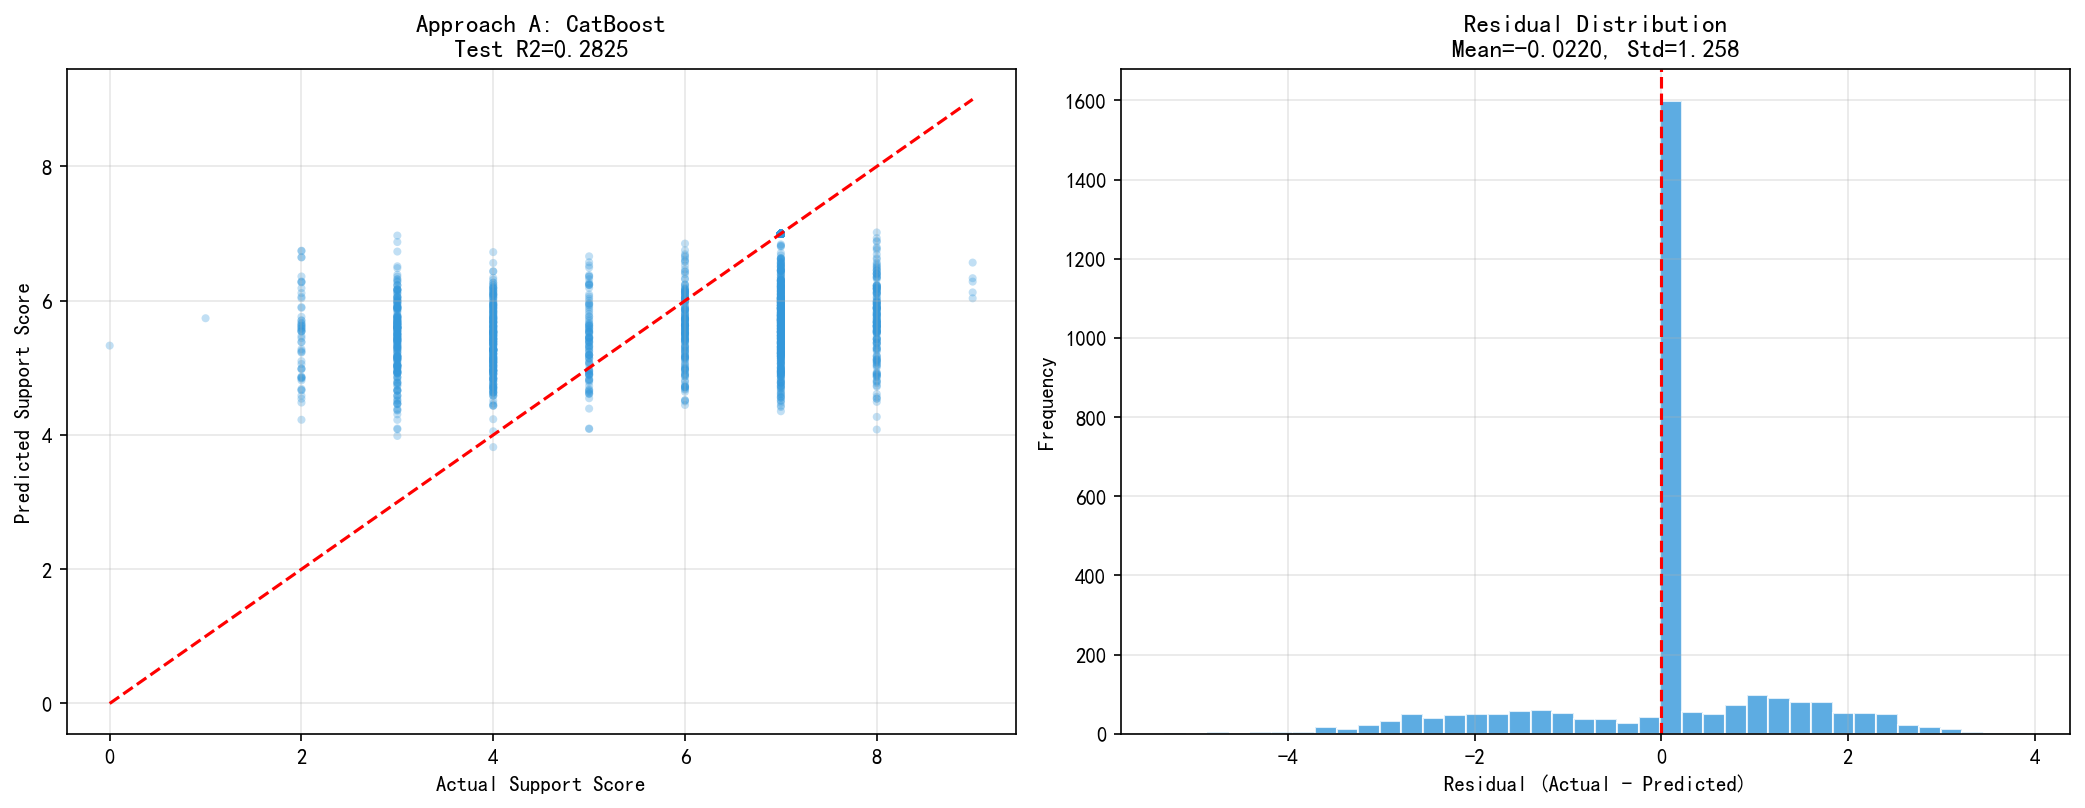
\includegraphics[width=0.95\textwidth]{figures/actual_vs_predicted.png}
    \caption{Predicted vs.\ actual support scores (left) and residual distribution (right).}
    \label{fig:actual_vs_predicted}
\end{figure}

\begin{figure}[H]
    \centering
    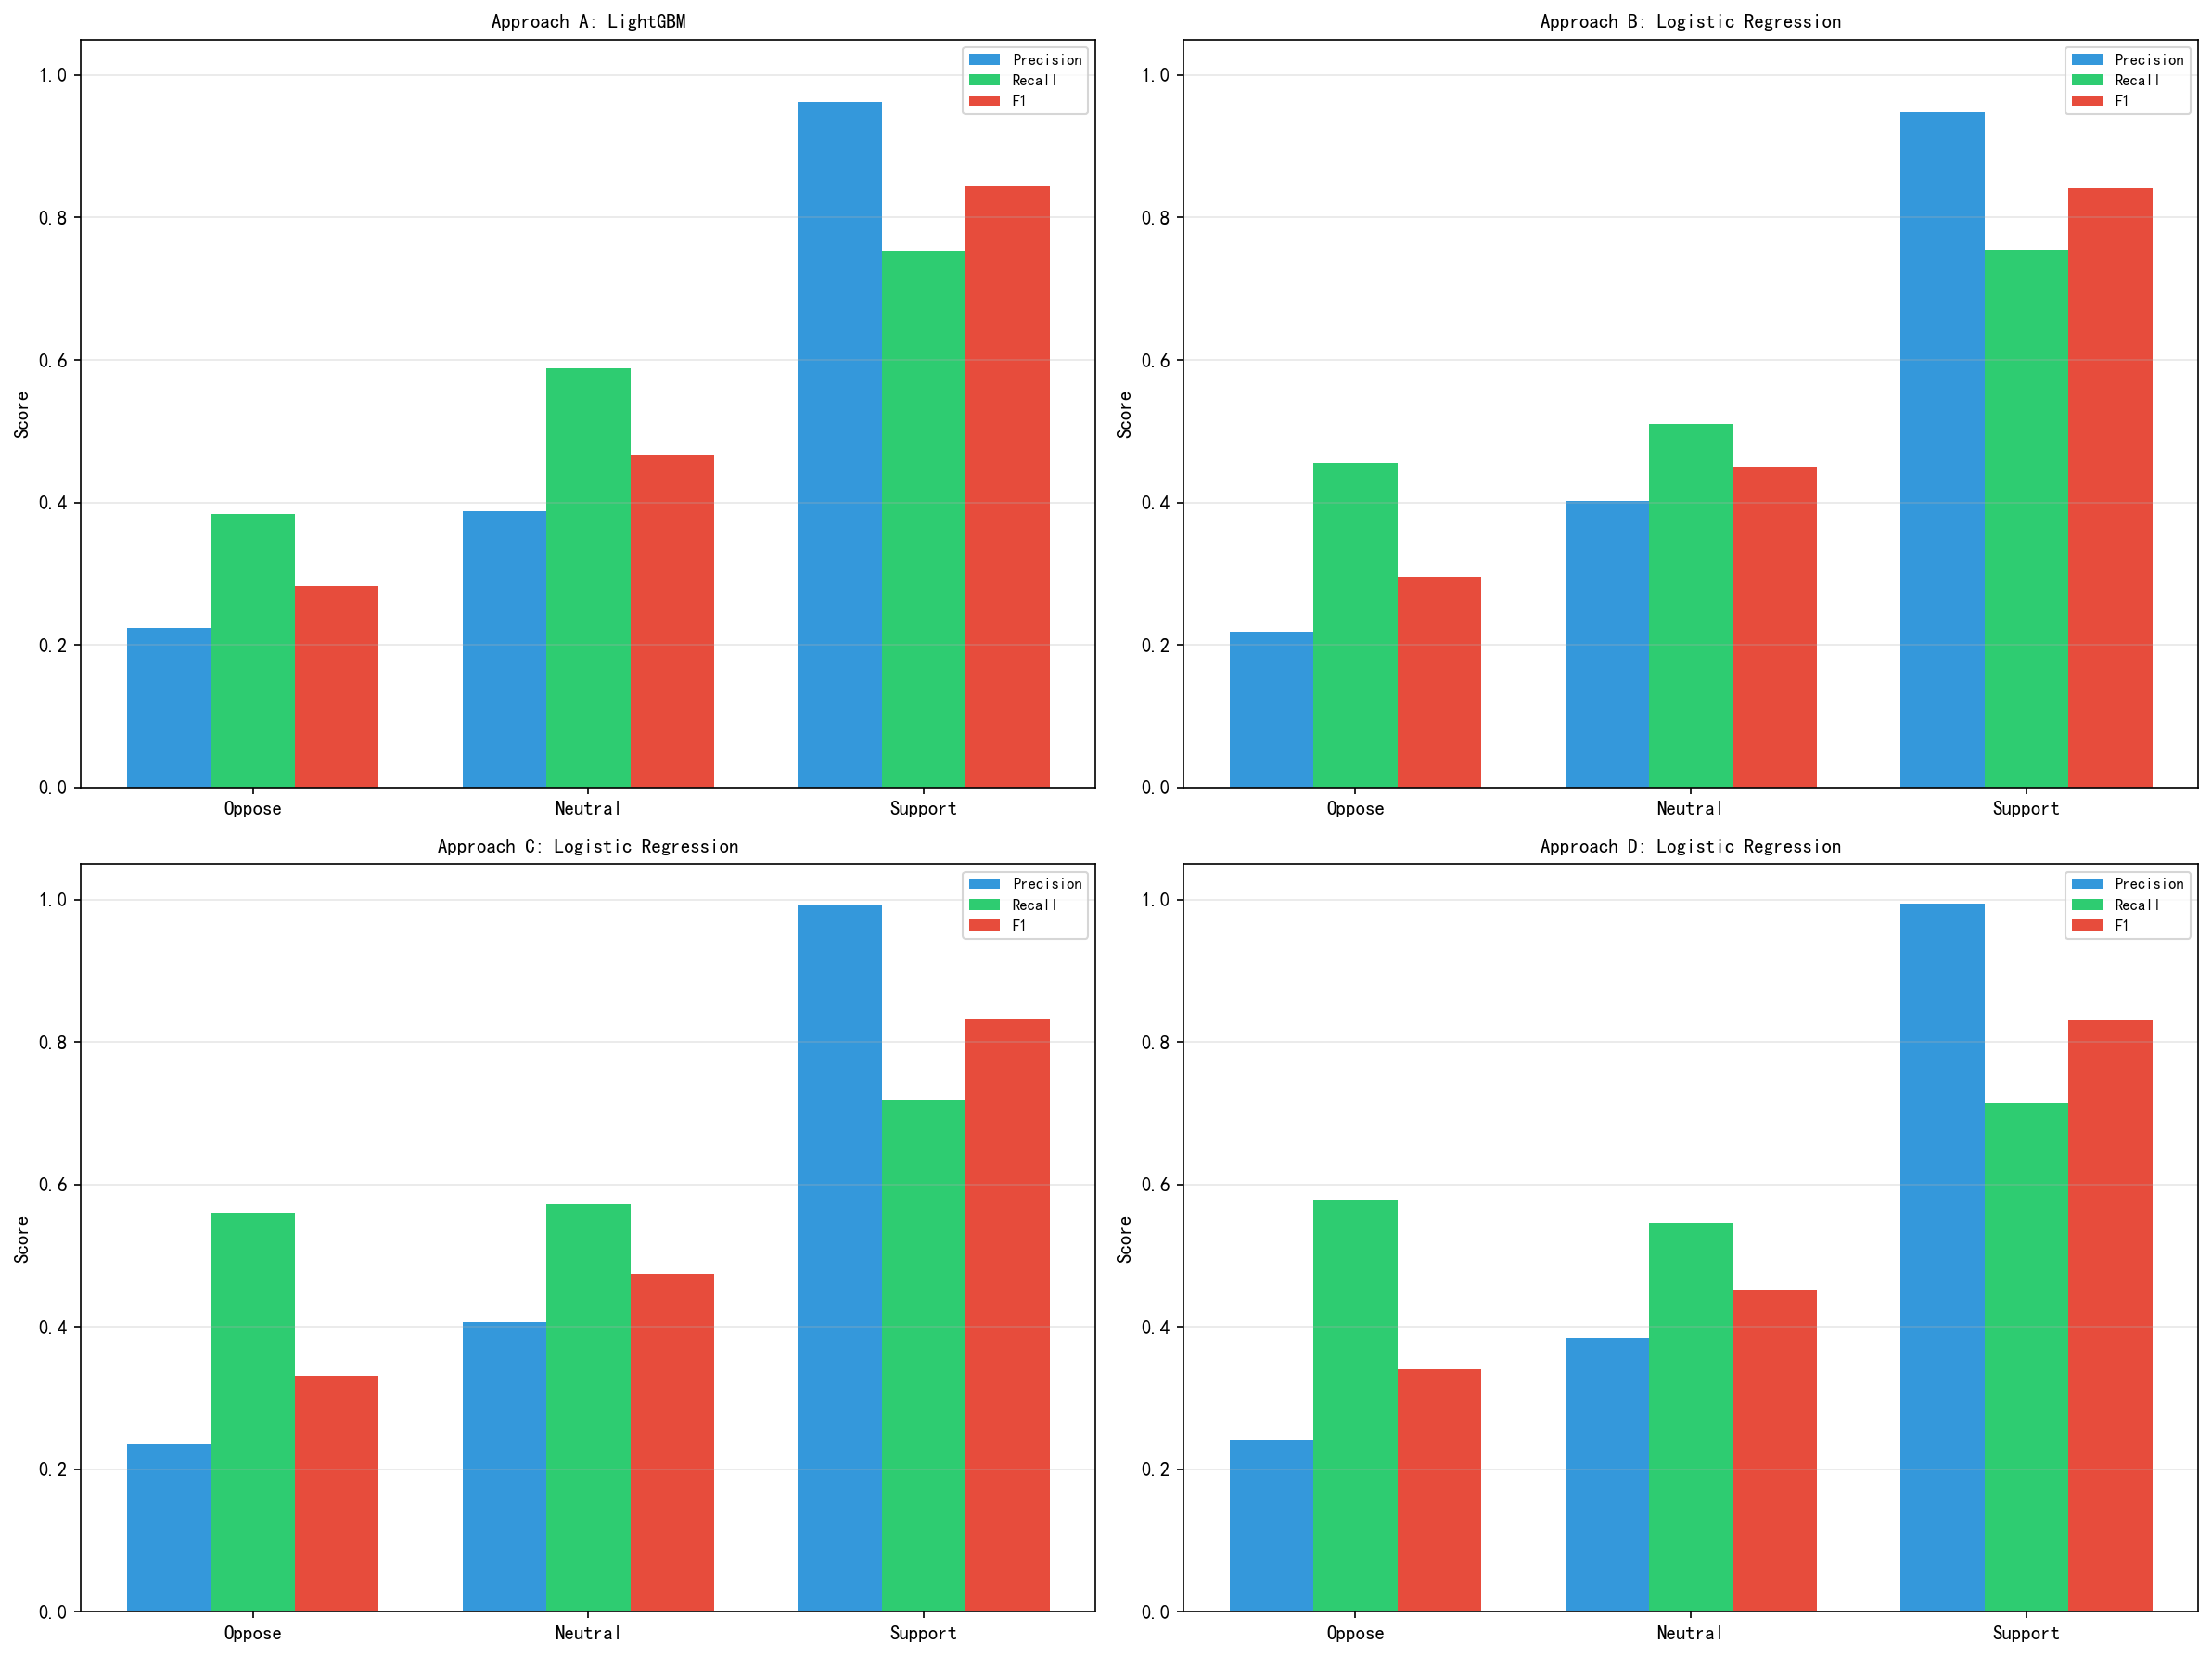
\includegraphics[width=0.95\textwidth]{figures/per_class_metrics.png}
    \caption{Per-class precision, recall, and F1 under the best classifier per approach.}
    \label{fig:per_class_metrics}
\end{figure}

\begin{figure}[H]
    \centering
    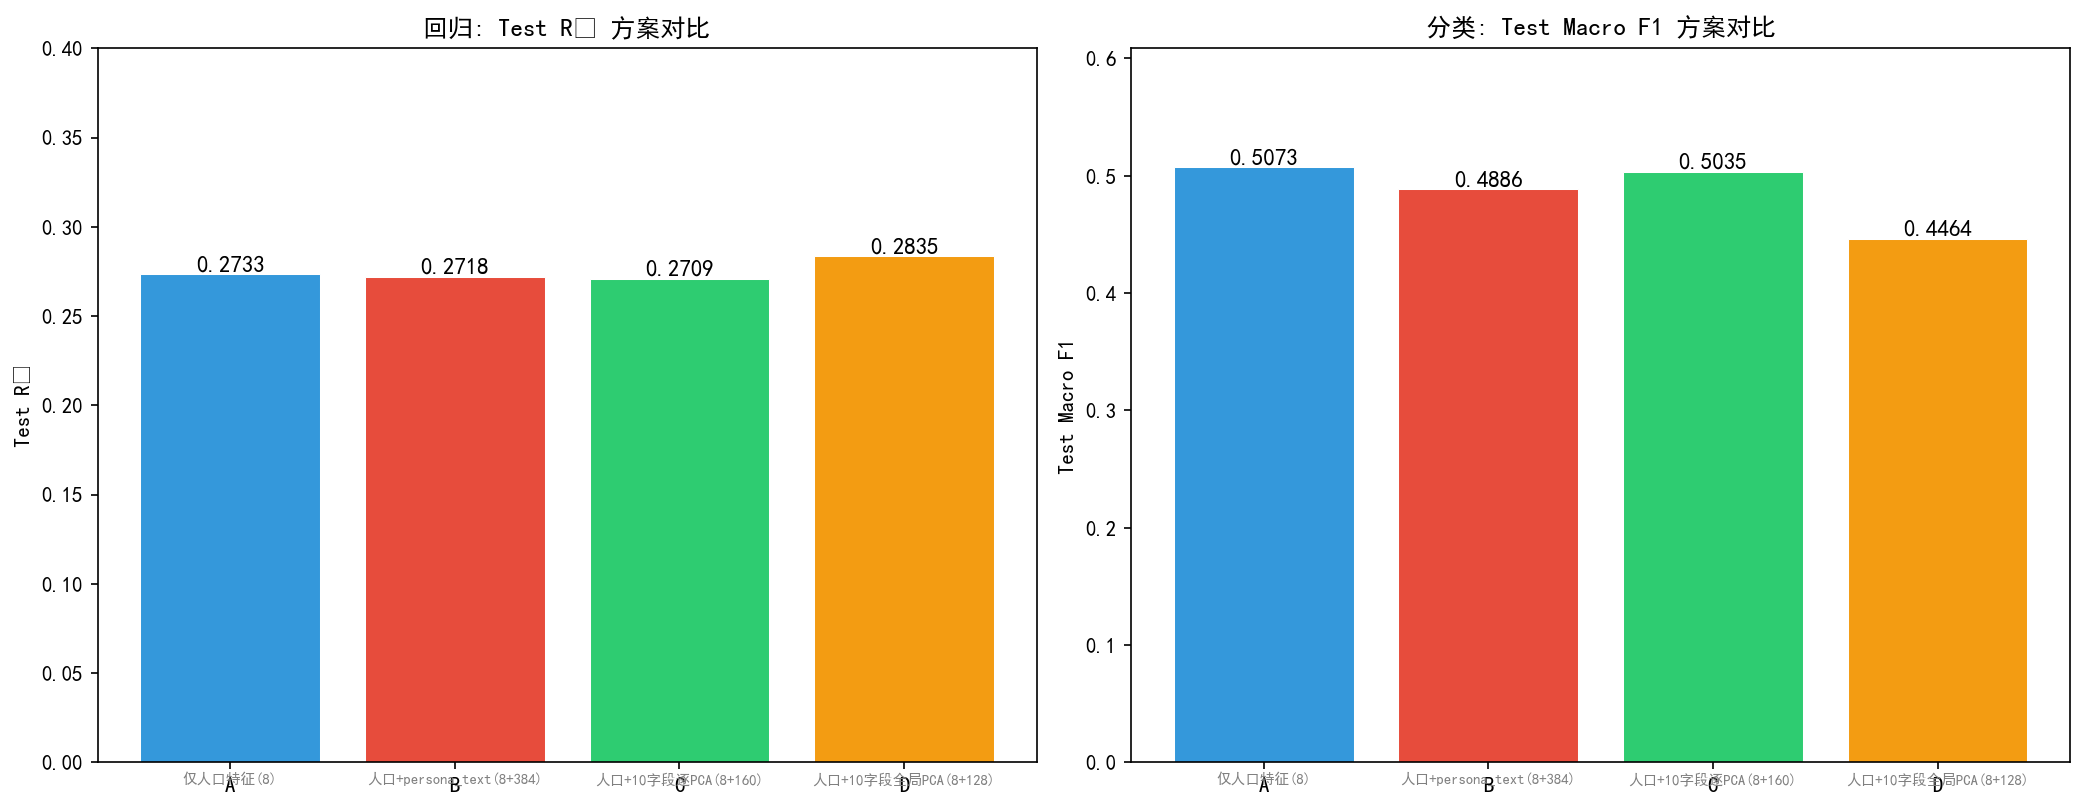
\includegraphics[width=0.95\textwidth]{figures/approach_comparison.png}
    \caption{Test set performance comparison across four feature approaches. Left: regression Test R$^2$; Right: classification Test Macro F1.}
    \label{fig:approach_comparison}
\end{figure}

\begin{figure}[H]
    \centering
    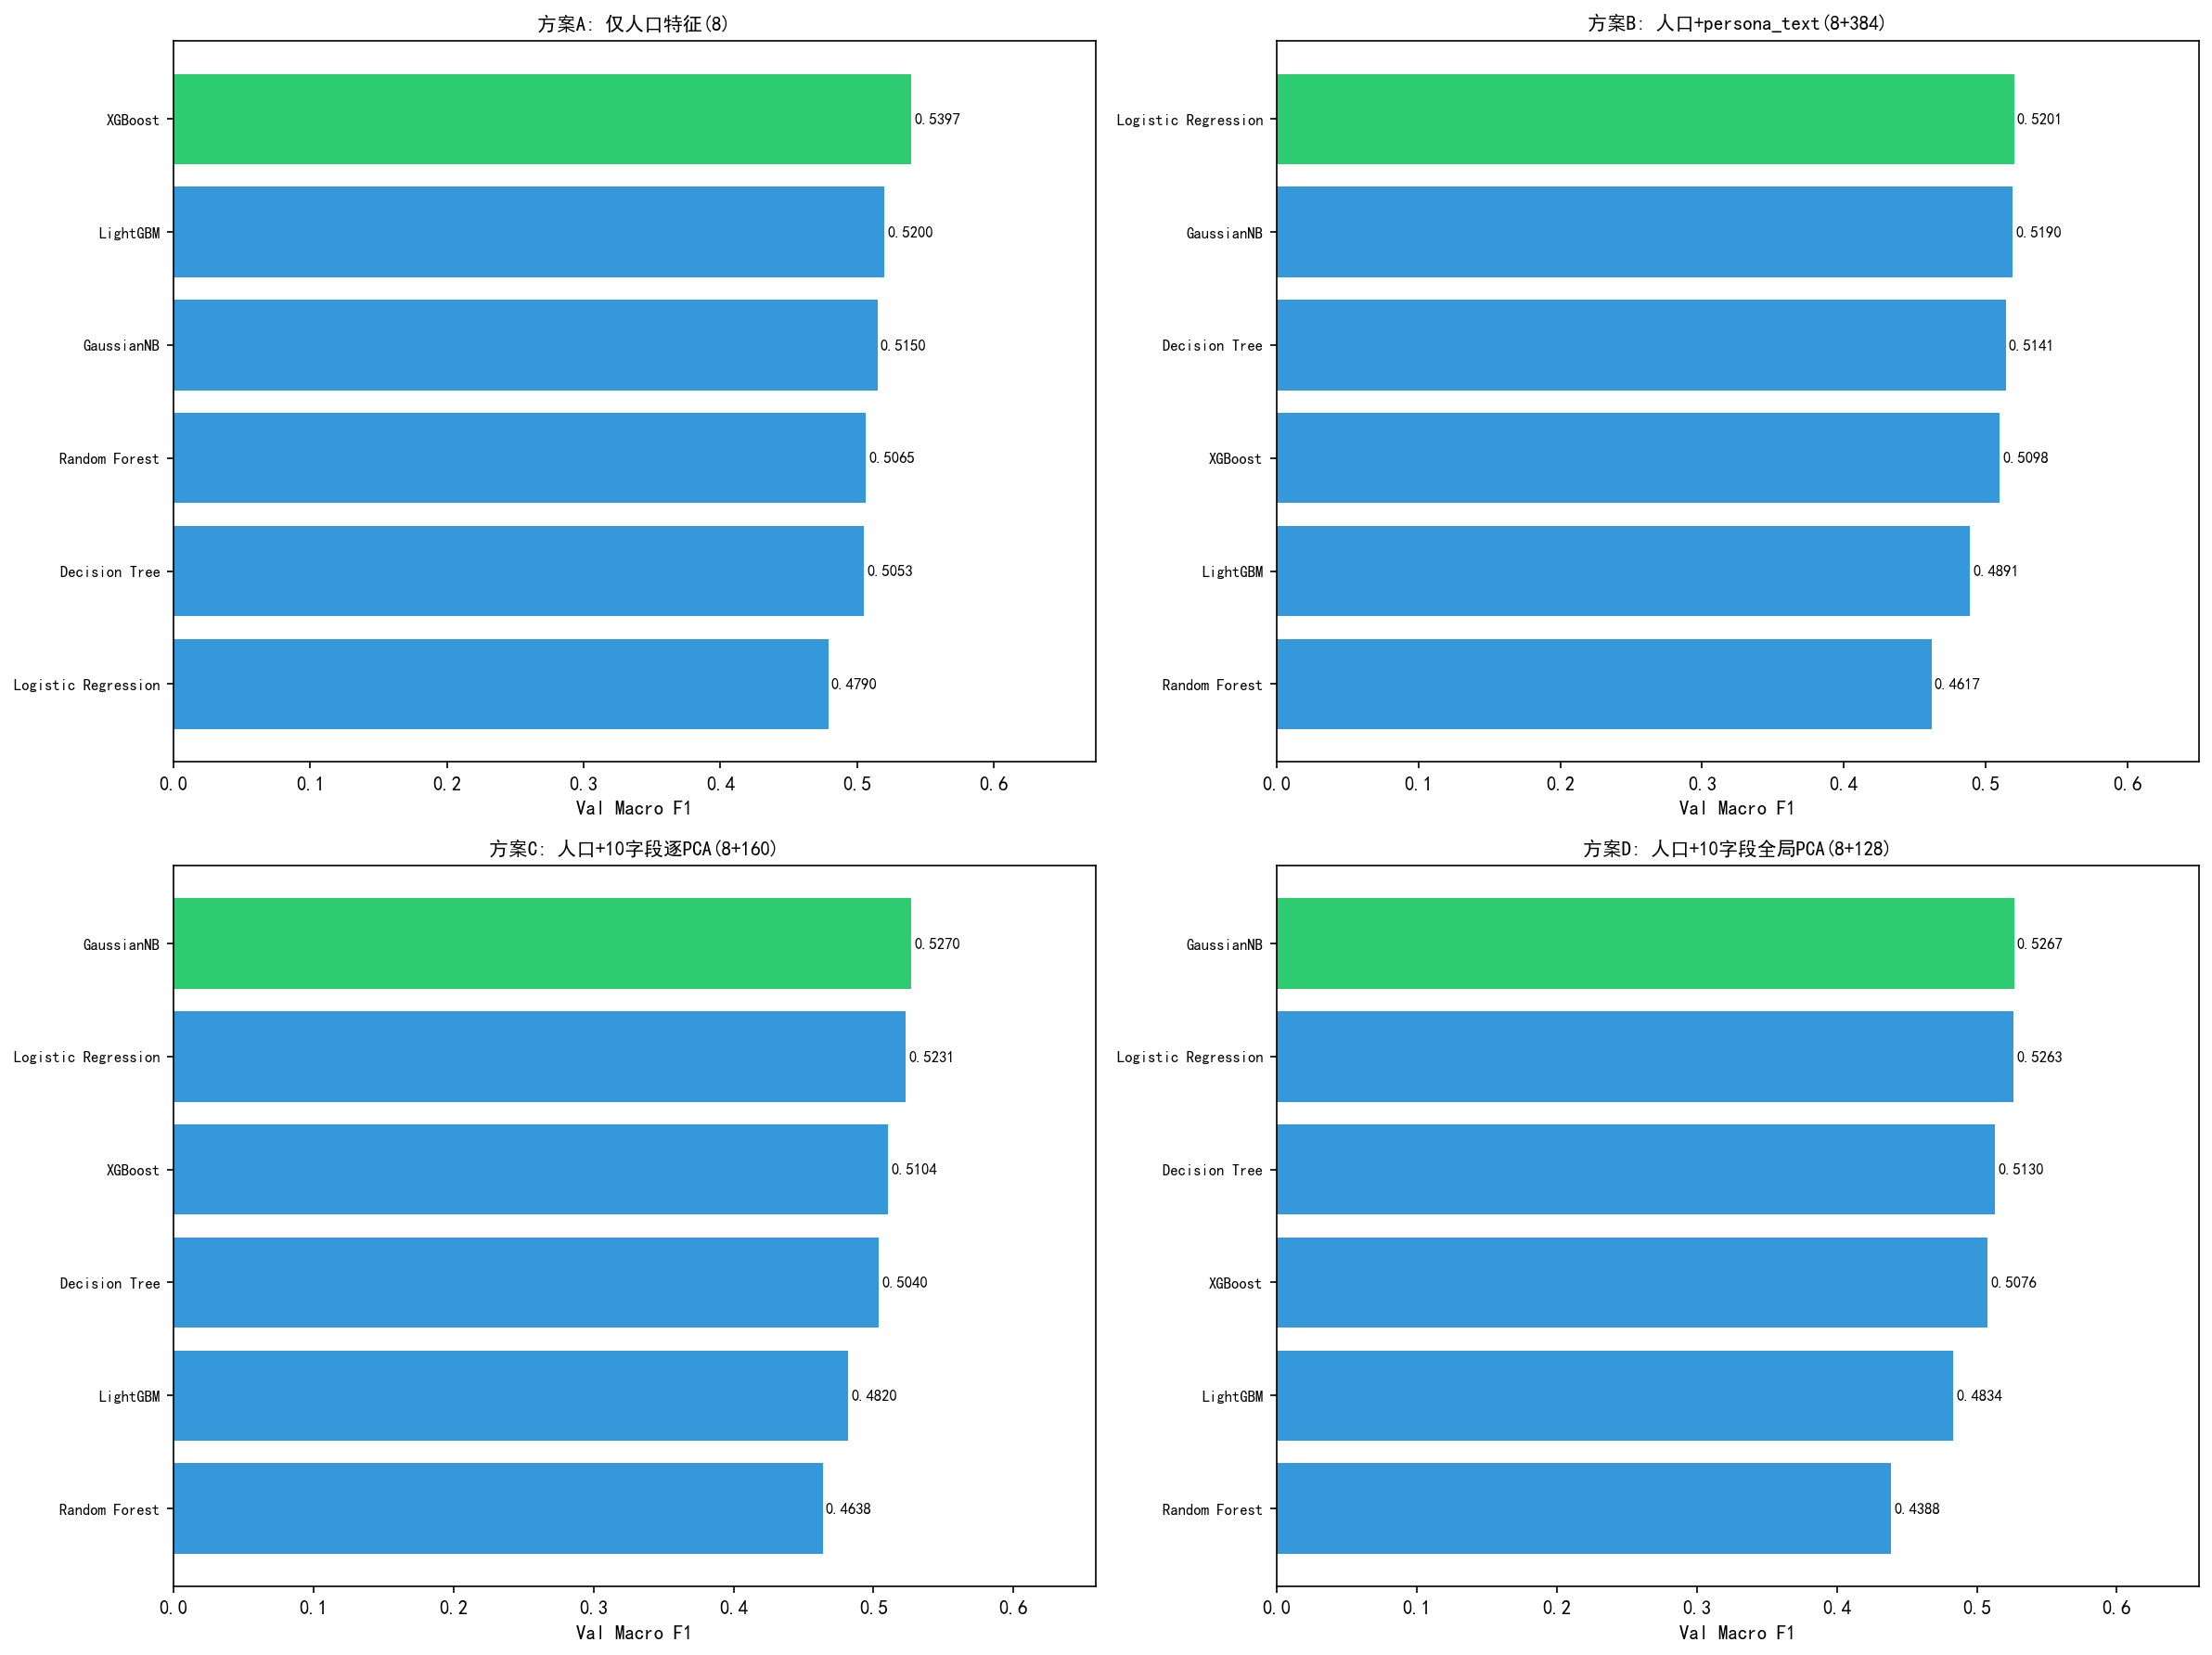
\includegraphics[width=0.95\textwidth]{figures/classification_by_approach.png}
    \caption{Classification Val Macro F1 by approach and model type.}
    \label{fig:classification_by_approach}
\end{figure}

\begin{figure}[H]
    \centering
    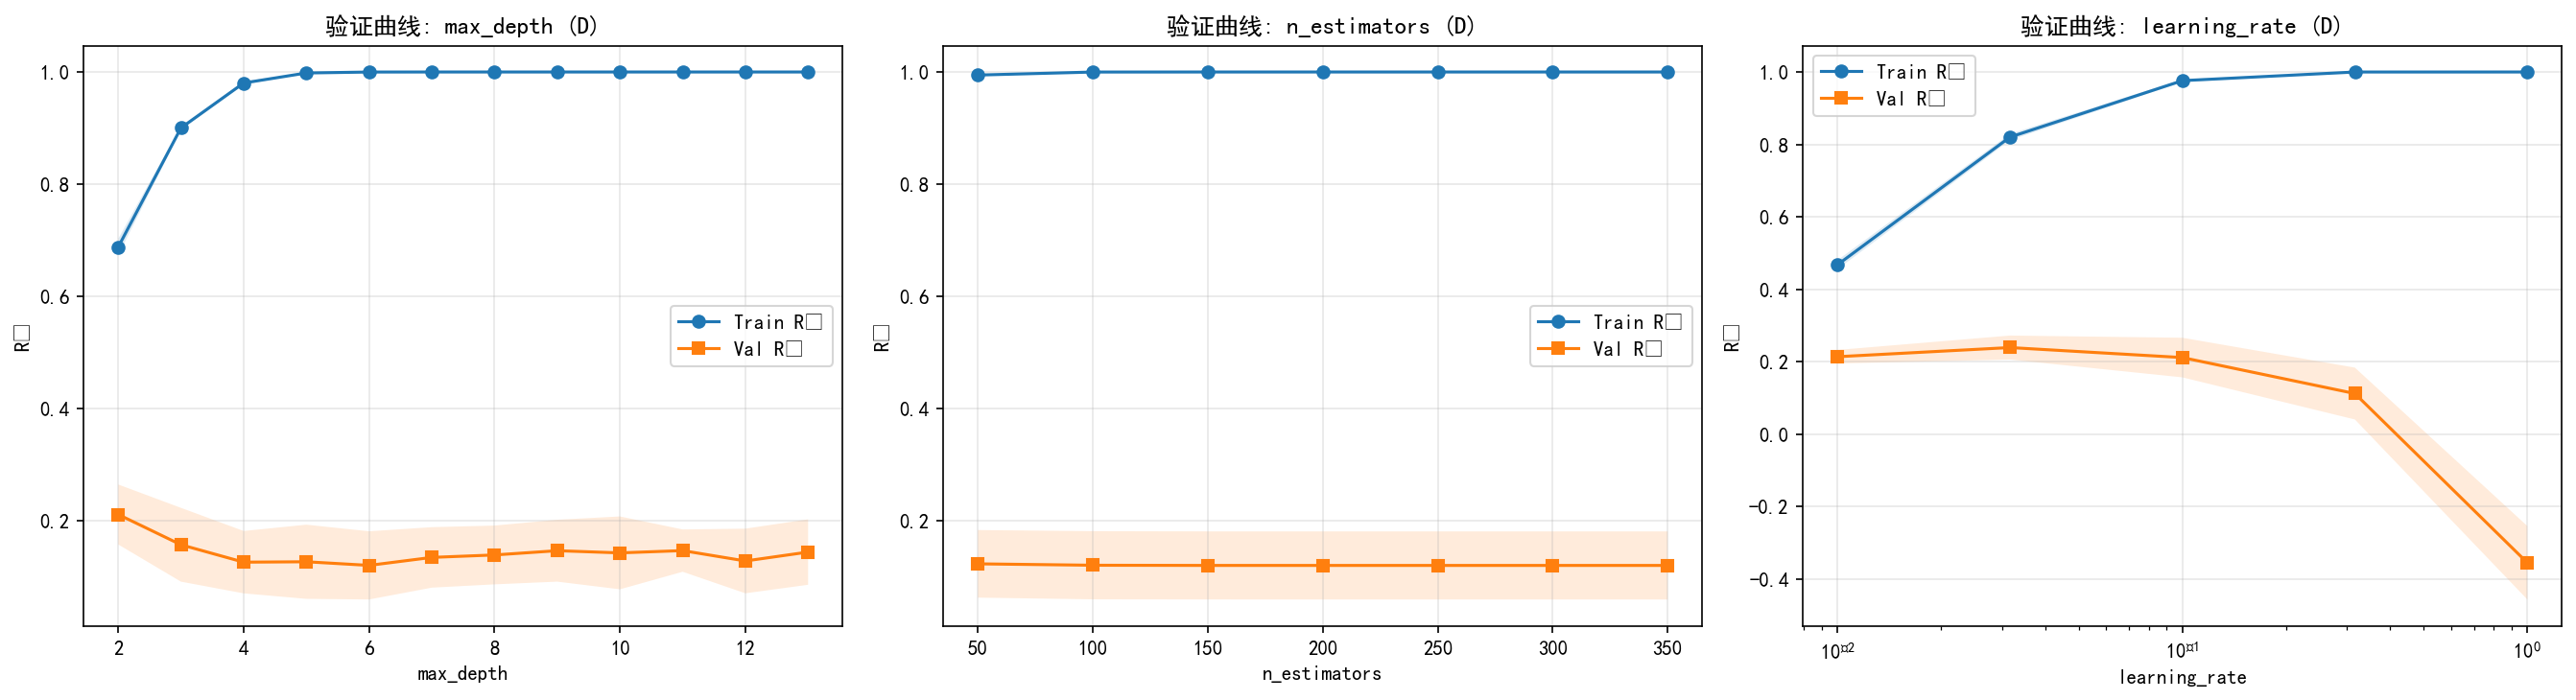
\includegraphics[width=0.95\textwidth]{figures/validation_curves.png}
    \caption{Validation curves for XGBoost hyperparameters (best approach).}
    \label{fig:validation_curves}
\end{figure}

\end{document}
